\chapter{Structural Perturbation of Lipid Bilayers Due to Tat Peptide}
%First, we discuss the results and analysis of diffuse X-ray scattering. The
%general protocol was the following; LAXS data were fitted to a model X-ray
%scattering pattern from a stack of fluctuating membranes via NFIT program,
%the analysis of which yielded the bending modulus, $K_C$, and the bulk
%modulus, $B$. Dividing the experimental data by the model, then, gave the 
%absolute X-ray form factor, $|F(q_z)$, which is the Fourier transform
%of bilayer electron density profile along the bilayer normal direction, $z$. 
%We fitted $|F(q_z)|$ to a model density profile using the scattering density
%profile (SDP) program. The SDP program allows us to model a bilayer density
%according to volumetric spacing constraint. The advantage of this program is
%that we can see fine details of bilayer structure such as an individual
%head group, terminal methyl, and so on. The model requires many parameters
%that are not so well determined. We then constrain many parameters from
%the past experimental data and MD simulations. This is discussed in 
%section ?.
%
%The second main method is MD simulation. From simulation trajectory, we 
%calculated the so called simulated X-ray form factor using the SIMtoEXP
%program (ref). The best matching simulation result was chosen as the best
%prediction of the bilayer structure. We, then, calculated many structural
%details from the trajectory that were not accessible experimentally.   
%
%Section X discusses the implication of the results obtained in the proceeding 
%sections. While this study does not probe dynamics of Tat translocation,
%it supports Tat's ability to interact with neutral membranes. This finding
%is compared with recent studies on a single arginine molecule.

%%%%%%%%%%%%%%%%%%%%%%%%%%%%%%%%%%%%%%%%%%%%%%%%%%%%%%%%%%%%%%%%%%%%%%%%%%%%%%%
\section{Introduction}\label{sec:Tat_intro}
The name cell-penetrating peptide (CPP) connotes a peptide that 
easily penetrates cell membranes (for Reviews see \cite{Fischer05,Joliot04,Lindgren00}). 

This thesis focuses on 
the transactivator of translation, Tat, from the HIV-1 virus, which plays a 
role in AIDS progression. Earlier work showed that the HIV-Tat 
protein (86 amino acids) was efficiently taken up by cells, and concentrations 
as low as 1 nM were sufficient to transactivate a reporter gene expressed from 
the HIV-1 promoter \cite{Frankel88,Green88}. 
It has been reported that Tat protein uptake does not 
require ATP \cite{Vives97}. 
Studies using inhibitors of different types of endocytosis, 
including clathrin and caveolae-mediated, or receptor-independent 
macropinocytosis reached the same conclusion that ATP mediated endocytosis is 
not involved in Tat protein permeation 
\cite{Ter-Avetisyan09,Duchardt07,Tunnemann06,Ziegler05}. 
However, this issue is 
controversial, as other studies found evidence for endocytosis in Tat protein 
import \cite{Wadia04,Kaplan05,Mann91,Richard05,Jones05,Vendeville04,Foerg05,Fittipaldi05,Liu00}. 
Still other studies have concluded that an ATP requirement for 
Tat protein entry depends on the size of the cargo attached to Tat protein, or 
on the specific cell type \cite{Torchilin01,Torchilin03,Rudolph03}. 
The part of the Tat protein responsible for 
cellular uptake was assigned to a short region Tat (48-60), G$_48$RKKRRQRRRPPQ$_60$, 
which is particularly rich in basic amino acids \cite{Vives97}. 
Deletion of three out of 
eight positive charges in this region caused loss of its ability to translocate 
\cite{Vives97}. 
In this chapter, short basic regions will be called Tat, while the 
entire 86 amino acid protein will be called Tat protein. 
Tat was shown to be responsible for the Tat
protein’s permeation into the cell nucleus and the nucleoli \cite{Vives97}, 
and this was confirmed using live cell fluorescence in SVGA cells \cite{Chauhan07}. 
Tat (48-60) was shown to have little toxicity on HeLa cells at 100 $mu$M 
concentration \cite{Vives97}, but the longer Tat protein (2-86) was toxic 
to rat brain glioma cells at 1-10 $mu$M \cite{Sabatier91}. 
Interestingly, no hemolytic activity was found when human erythrocytes
were incubated with a highly neurotoxic concentration (40 $mu$M) of Tat (2-86) 
\cite{Sabatier91}. 
These results prompt the question, what is the mechanism of Tat’s translocation through 
membranes?
To address this question, many biophysical studies have used simple models of
biological membranes composed of a small number of lipid types. These studies 
are valuable
because there is no possibility for ATP-dependent translocation, thus ruling 
out endocytosis if
translocation occurs. For example, Mishra et al. reported that the rate of 
entry into giant
unilamellar vesicles (GUVs) composed of PS/PC (1:4 mole ratio) lipids of 
rhodamine-tagged Tat
is immeasurably slow, but it crosses a GUV composed of PS/PC/PE (1:2:1) lipids 
within 30
seconds \cite{Mishra08}. 
This study suggests that negative curvature induced by the 
inclusion of PE facilitates translocation. 
In a subsequent study using much smaller unilamellar vesicles (LUVs),
Tat did not release an encapsulated fluorescent probe in LUVs composed of 
lipids modeling the outer plasma membrane, PC/PE/SM/Chol (1:1:1:1.5), 
but did release the probe in LUVs composed of BMP/PC/PE (77:19:4) \cite{Yang10}; 
BMP (bis(monoacylglycero)-phosphate) is an anionic lipid specific to late 
endosomes. In that study \cite{Yang10}, the inclusion of PE did not suffice to 
cause leaky fusion in LUVs in the absence of a negatively charged lipid. The 
contrasting results in these two experiments may also be due to the use of LUVs 
instead of GUVs since it was reported that Tat does not translocate across LUVS 
of PC/PG (3:2) but does translocate across GUVs of the same lipid composition 
\cite{Thoren04}. In a similar experiment, Tat did not translocate into egg PC
LUVs \cite{Kramer03}. In another experiment confirming these results, Tat did 
not translocate into GUVs containing only PC with 20 mol\% cholesterol, but 
when PS or PE was included with PC, then rapid translocation of Tat was observed 
\cite{Ciobanasu10}. These experiments demonstrate that the choice of lipids and 
model systems influences Tat translocation.

Is a pore formed during Tat translocation? Although direct conductance 
measurements of Tat and lipid membranes have not been carried out, two studies 
measured conductance with the somewhat similar CPP oligoarginine R$_9$C peptide. 
Using single-channel conductance of gramicidin A in planar lipid membranes 
consisting of anionic, neutral or positively charged lipids, R$_9$C did not 
increase conductance, even in anionic lipid membranes \cite{Gurnev13}. 
By contrast, in a similar experiment using planar lipid membranes, a current 
was induced by R$_9$C in PC/PG (3:1) membranes, with increasing destabilization 
over time \cite{Herce09}. Thus questions remain about pore formation of Tat in 
membranes. In the GUV experiment with Tat mentioned above \cite{Ciobanasu10},
Ciobanasu \textit{et al.}, using size exclusion methods, suggested a pore in the 
nanometer range, which could only be passed by small dye tracer molecules. Thus, 
if a true pore forms, it is likely to be small and transitory.

The secondary structure of Tat has been characterized by many researchers. 
Ref.\cite{Thoren04} carried out Circular dichroism (CD) spectroscopy on a 
variation of Tat where the penultimate proline on Tat (48-60) was replaced by a
tryptophan \cite{Thoren04}. Their study found a random coil secondary structure 
in aqueous solution as well as when Tat was mixed with PC/PG/PE (65:35:5) LUVs. 
Ziegler \textit{et al.} \cite{Ziegler05} obtained the same result using CD in 
PC/PG (3:1) vesicles. In addition, solid state NMR has identified a random coil 
structure of Tat in DMPC/DMPG (8:7 mole ratio) multibilayers \cite{Su10}. 
In the larger Tat-(1-72)-protein NMR measurements at pH 4 have determined there 
is no secondary structure, with a dynamical basic region \cite{Shojania06}. 
Similarly, NMR was used to study the full Tat protein and found a highly 
flexible basic region \cite{Bayer95}. These previous studies indicate that 
an alpha helix is not required for Tat’s translocation ability. 

Regarding the mechanism of translocation of this randomly structured, short 
basic peptide, many models have been proposed based on the conflicting results 
listed above. Molecular dynamics simulations offer some insight into the 
molecular details of translocation. Herce and Garcia simulated the 
translocation of Tat (Y$_{47}$GRKKRRQRRR$_{57}$) across DOPC at various 
lipid:peptide molar ratios \cite{Herce07}. Their simulations indicated that Tat 
binds to the phosphate headgroups, with 1 Tat binding with 14 lipids, each 
positive charge on Tat associated with nearly 2 phosphate groups \cite{Herce07}. 
Translocation involved a localized thinning, and snorkeling of arginine side 
chains through the hydrophobic layer to interact with phosphates on
the other side of the membrane. This allowed some water molecules to penetrate 
the membrane along with Tat, forming a pore \cite{Herce07}. In this simulation, 
performed without inclusion of counterions, pore formation was only observed at 
high ratios of peptide:lipid (1:18) or at elevated temperature. However, a 
subsequent Gromacs simulation with counterions found no thinning and no pore 
formation when Tat was added to DOPC membranes \cite{Yesylevskyy09}. Instead it 
found a membrane invagination associated with a cluster of Tat peptides. From 
their findings, the authors suggested that micropinocytosis could be the model 
for Tat translocation across membranes \cite{Yesylevskyy09}. 

In this thesis, I combine experimental low-angle X-ray scattering (LAXS) 
data with MD simulations to obtain the structure of fully hydrated, oriented 
lipid bilayers with Tat (47-57) added at several mole ratios. The lipid systems 
were DOPC, DOPC/DOPE (3:1 mole ratio), DOPC/DOPS (3:1), DOPC/DOPE (1:1) and a 
mimic of the nuclear membrane (POPC/POPE/POPS/SoyPI/Chol, 69:15:2:4:11). 

%%%%%%%%%%%%%%%%%%%%%%%%%%%%%%%%%%%%%%%%%%%%%%%%%%%%%%%%%%%%%%%%%%%%%%%%%%%%%%%
\section{Materials and Methods}
\subsection{Volume Measurements}\label{sec:volume_method}
Multilamellar vesicles (MLVs) were prepared by mixing dried lipid mixtures with 
MilliQ water to a final concentration of 2-5 wt\% in nalgene vials and cycling 
three times between 20 \textcelsius\ and 60 \textcelsius\ for ten minutes at 
each temperature with vortexing. Pure Tat was dissolved in water at 0.4 wt\%.

Volumes of lipid mixtures with and without peptides in fully hydrated 
multilamellar vesicles (MLV) were determined at 37$\pm$ 0.01 \textcelsius\ 
using an Anton-Paar USA DMA5000M (Ashland, VA) vibrating tube densimeter. 
This instrument measures the average density of a solution and compares it to
the density of air using $\rho_s-\rho_0=k(\tau_s-\tau_0)^2$ where $k$ is
an instrumental ??? that depends on the atmospheric pressure. 

The Tat peptide sequence used in X-ray experiements and MD simulations was 
Y$_{47}$GRKKRRQRRR$_{57}$. Table~\ref{tb:aa} lists the chemical formulas and 
molecular weights of these amino acids for convenience. The molecular weight of 
this sequence is 
$181.2+75.1+146.1+2 \times 146.2+6\times 174.2-10\times 18=1560$.
The Tat peptides were synthesized in trifluoroacetic acid, which has 
the chemical formula $\mathrm{CF_3CO_2H}$, and is made into a powder form by the 
freeze-dry method. Therefore, each positively charged amino acid such as 
an arginine and lysine was counter-balanced by a trifluoroacetate (TFA)
($\mathrm{C_2F_3O_2}$). Since Tat has six arginines and two lysines, it came 
with eight trifluoroacetates. This complex has a molecular weight of 
$1560+113\times 8=2464$. We used the 
molecular weight of this complex in order to calculate the molarity of Tat
correctly. The same molecular weight was also used in preparing oriented 
samples.

\begin{table}[htbp]
  \centering
  \begin{tabular}{c c c c}
    \hline
    Code & Amino acid & Chemical Formula & Molecular weight \\
    & & & (g/mol) \\
    \hline
    K & Lysine & $\mathrm{C_6H_{14}N_2O_2}$ & 146.2 \\
    R & Arginine & $\mathrm{C_6H_{14}N_4O_2}$ & 174.2 \\
    G & Glycine & $\mathrm{C_2H_5NO_2}$ & 75.1\\
    Y & Tyrosine & $\mathrm{C_9H_{11}NO_3}$ & 181.2 \\
    Q & Glutamine & $\mathrm{C_5H_{10}N_2O_3}$ & 146.1 \\ 
    \hline
  \end{tabular}
  \caption{Some Amino Acids Data}
  \label{tb:aa}
\end{table}

The Tat volume $\VTat$ was calculated from the measured average density of a 
Tat-water solution in the following way. Assuming that Tat
molecules in water do not change the volume of water molecules, the density
of Tat-water solution is equal to the mass of Tat-water solution divided
by the sum of volumes of water and Tat, 
\begin{equation}
  \rho_\textrm{sol} = \frac{\mw+\mc}{\Vw+\Vc\Nc},
\end{equation}
where $\mw$ and $\mc$
are the total masses of water and Tat-TFA complex, respectively, 
$\Vw$ is the total volume of 
water, $\Vc$ is the molecular volume of a Tat-TFA complex, and $\Nc$ is the total number 
of this complex in the solution. 
Denoting $\Vw=\mw/\rho_\textrm{w}$ 
and $\Nc=N_\textrm{A}\mc/\Wc$, 
where $\Wc$ is the molecular weight of the complex, 
$N_\textrm{A}$ is the Avogadro's number,
and $\rho_\textrm{w}$ is the density of water, we have
\begin{equation}
  \Vc = \frac{\Wc}{\rho_\textrm{sol}N_\textrm{A}} \left( 
        1 + \frac{\mw}{\mc}\left(1-\frac{\rho_\textrm{sol}}{\rho_\textrm{w}}\right) 
        \right),
\end{equation}
which allows us to calculate the molecular volume of a Tat-TFA complex 
from the experimentally measured quantities. 
Assuming that the molecular
volume scales with the molecular weight gives the volume of Tat, 
$\VTat$ = $1560/2464\times\Vc$ \AA$^3$. 

%%%%%%%%%%%%%%%%%%%%%%%%%%%%%%%%%%%%%%%%%%%%%%%%%%%%%%%%%%%%%%%%%%%%%%%%%%%%%%%
\subsection{Analysis of Diffuse Scattering}
Figure~\ref{fig:figure1} shows our typical Low angle X-ray scattering (LAXS) data 
from oriented stacks of fluctuating bilayers in the fluid phase. Analysis of diffuse scattering 
intensity patterns like the one shown in Fig.~\ref{fig:figure1} results in material 
parameters such as the bending modulus $K_c$ and bulk modulus $B$ as well as
the absolute form factor $|F(q_z)$. 
The form factor is the Fourier transform of the bilayer electron 
density profile $\rho(z)$ and gives us information about the internal structure of the
bilayers interacting with Tat peptides.

\begin{figure}[htbp]
  \centering
  \includegraphics[width=0.5\textwidth]{figures/Tat/figure1}
  \caption{LAXS of DOPC:DOPE (1:1) with $\xTat$ = 0.034 at 37 \textcelsius. 
  White lobes of diffuse scattering intensity have large grey numbers, while
  lamellar orders and beam are shown to the left of the
  molybdenum beam attenuator (short, dark rectangle). $q_z$ and $q_r$ are the 
  cylindrical coordinates of the sample $q$-space, where $q_z$-axis is along 
  the bilayer normal and $q_r$-axis is along the in-plane direction. 
  The lamellar repeat spacing was $D$ = 66.2 \AA.}
  \label{fig:figure1}
\end{figure}

The form factor $F(q_z)$ is obtained by realizing that the diffuse scattering
intensity pattern $I(\mathbf{q})$ is a product of the structure factor $S(\mathbf{q})$ and
the form factor; $I(\mathbf{q})= S(\mathbf{q})|F(q_z)|^2$. This means that 
once the two dimensional structure factor map $S(\mathbf{q})$ is calculated 
from a model free energy for bilayer fluctuations, the form factor can simply
be calculated by dividing the intensity by the structure factor. 
Getting the best fit of a model structure factor to the intensity results in 
the material parameters, $K_c$ and $B$.

We used an analysis program called NFIT developed by Dr. Yufeng Liu
\cite{Lyatskaya01,Liu04,Liu03} to analyze the diffuse scattering and
obtain the bending modulus, bulk modulus, and form factor. 
The details of the analysis are found in Dr. Yufeng Liu's thesis 
\cite{Liu03}. This section outlines the method. 

X-ray scattering essentially reflects the electron density distribution
of the sample system. This includes not only the average electron
density but also the disorder caused by fluctuations about the average.
In our samples, the electron density distribution reflects
the stacking of the bilayers, whose average structure can be described
as a one-dimensional array of membranes, each of which is a two-dimensional
in-plane fluid. A sketch of the membrane stack is shown in Fig.~\ref{fig:stack}.

\begin{figure}[htbp]
  \centering
  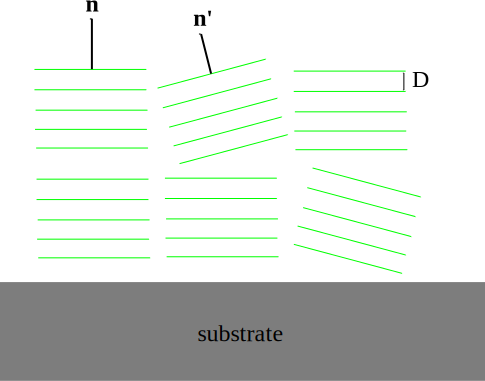
\includegraphics[width=0.5\textwidth]{figures/Tat/stack}
  \caption{Schematic of an oriented stack of lipid bilayers. Thick green curves
  represent an instance of thermally fluctuating bilayers. The dashed lines 
  show the thermally averaged positions $z=nD$ of the centers of each bilayer 
  and $u_{n}(x,y)$ gives the instantaneous deviation from the average. 
  Each bilayer extends in the $\mathbf{r}=\left(x,y\right)$ plane.}
  \label{fig:stack}
\end{figure}

Fluctuations in the stack of the bilayers are described by the
quantities $u_{n}\left(\mathbf{r}\right)$, which are the spatial
deviations of the center of the $n$-th bilayer 
from its average position in the $z$ direction
at the in-plane location $\mathbf{r}=(x,y)$.
Given this description of structure of the lipid bilayer system, we
write the electron density $\rho _{n}$ of the $n$-th bilayer as 
\begin{equation}
  \rho_n(z,r) = \rho(z-nD-u_{n}(\mathbf{r}))
  \label{eq:rho1}
\end{equation}
where $\rho(z)$ is the electron density profile of a single, flat 
(no fluctuations) bilayer centered at $z=0$ with its normal in the 
$z$ direction. Eq.~(\ref{eq:rho1}) is not quite accurate for an incompressible
fluid phase bilayers because it ignores the $\cos\alpha$ factor \cite{Liu03} 
(see Fig.~\ref{fig:stack2}). To correct for the absence of this factor, 
the undulation correction \cite{Nagle00} was applied to all our 
form factors in this thesis. For a typical sample, this correction is about 
2\% \cite{Liu03}. We then write the electron density of a stack of $N$ bilayers,
\begin{equation}
  \rho \left(\mathbf{R}\right)=\sum _{n=0}^{N-1}\rho _{n}\left(z,\mathbf{r}\right).
  \label{eq:rho3}
\end{equation}

\begin{figure}[htbp]
  \centering
  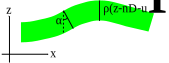
\includegraphics[width=0.5\textwidth]{figures/Tat/stack2}
  \caption{Expanded view of a fluctuating bilayer. Along the two black solid
  lines, the electron density profile is identical in an incompressible 
  bilayer. Along the dashed line, the bilayer appears thicker by a factor
  $1/\cos\alpha$. This apparent thickness variation along the $z$ direction 
  is corrected by the undulation correction.}
  \label{fig:stack2}
\end{figure}

Basic X-ray scattering theory in the usual Born approximation gives
\begin{align}
  I\left(\mathbf{q}\right) &\propto \int d\mathbf{R}d\mathbf{R}' 
  \rho(\mathbf{R})\rho (\mathbf{R}')e^{i\mathbf{q}\cdot (\mathbf{R}-\mathbf{R}')}\nonumber \\
  & = \left|\int_V d^{3}\mathbf{R} \rho \left(\mathbf{R}\right)e^{i\mathbf{q}\cdot \mathbf{R}}
  \right|^{2},\label{eq:eq1}
\end{align}
where $\rho \left(\mathbf{R}\right)$ is the electron density distribution
function of a stack of bilayers. 
Because X-ray scattering measures integrated intensity over time, 
Eq.~(\ref{eq:eq1}) requires thermal averaging indicated by angular brackets, 
\begin{equation}
  I\left(\mathbf{q}\right)=\left\langle \left|\int _{V}\rho \left(\mathbf{R}\right)e^{i\mathbf{q}\cdot \mathbf{R}}d^{3}\mathbf{R}\right|^{2}\right\rangle .\label{eq:int2}
\end{equation}
Using Eq.~(\ref{eq:rho1}) and (\ref{eq:rho3}), it can be shown that \cite{Liu03}
\begin{equation}
  I\left(\mathbf{q}\right) = \left|F(q_{z})\right|^{2}S\left(\mathbf{q}\right)
  \label{eq:factor1}
\end{equation}
where
\begin{equation}
  S\left(\mathbf{q}\right)=\left\langle \left|\sum _{n=0}^{N-1}\int e^{inDq_{z}+iu_{n}\left(\mathbf{r}\right)q_{z}+i\mathbf{q}_{r}\cdot \mathbf{r}}d^{2}\mathbf{r}\right|^{2}\right\rangle,
  \label{eq:sq0}
\end{equation}
and
\begin{eqnarray}
  F(q_{z}) & = & \int _{V}\rho \left(z\right)e^{iq_{z}z}dz\nonumber \\
  & = & \int \rho \left(z\right)\cos (q_{z}z)dz.
  \label{eq:form_factor}
\end{eqnarray}
The second equality in Eq.~(\ref{eq:form_factor}) follows for centro-symmetric lipid bilayers.
Assuming that $u_n(\mathbf{r})-u_m(\mathbf{r'})$ has a normal distribution,
we write Eq.~(\ref{eq:sq0}) as
\begin{eqnarray}
  S\left(\mathbf{q}\right) & = & \sum _{n,m=0}^{N-1}e^{iq_{z}(n-m)D}\int _{V}d^{2}\mathbf{r}d^{2}\mathbf{r}^{\prime }e^{i\mathbf{q}_{r}\cdot \left(\mathbf{r-r}^{\prime }\right)}G(r,r',n,m),
  \label{eq:struct2}
\end{eqnarray}
where 
\begin{eqnarray}
  G & = & \left\langle e^{iq_{z}\left(u_{n}\left(\mathbf{r}\right)-u_{m}(\mathbf{r}')\right)}\right\rangle \nonumber \\
  & \approx & e^{-\frac{q_{z}^{2}\left\langle \left[u_{n}\left(\mathbf{r}\right)-u_{m}(\mathbf{r}')\right]^{2}\right\rangle }{2}\; .}
  \label{eq:G}
\end{eqnarray}
$G$ is called the scattering pair correlation function. The second approximation 
is obtained by employing the harmonic approximation \cite{Liu03}. 
Eq.~(\ref{eq:struct2}) is an general expression for a system whose electron
density distribution has the form given by Eq.~(\ref{eq:rho1}) and (\ref{eq:rho3}).

The membrane fluctuations given by $\left\langle\bracks{u_n(\mathbf{r})-u_m(\mathbf{r'})}^2\right\rangle$ 
in Eq.~(\ref{eq:G}) are calculated from the free energy functional 
for smectic liquid crystals. The basic degrees of freedom in this free energy
include (1) bending of each membrane independently of others in the
stack and (2) interactions between membranes in the stack. The bending
free energy is proportional to the curvature squared with a bending
modulus $K_{c}$ as shown in the first term in the following free energy equation
\begin{equation}
  F_{U}=\frac{1}{2}\int d\mathbf{r}\sum _{n=0}^{N-1}\left\{ 
  K_{c} \left[\nabla _{r}^{2}u_{n}\left(\mathbf{r}\right)\right]^{2}
  +B\left[u_{n+1}\left(\mathbf{r}\right)-u_{n}\left(\mathbf{r}\right)\right]^{2}
  \right\}.
  \label{eq:free_energy}
\end{equation}
The second term is a harmonic approximation to the interactions between
membranes with a modulus $B$. From analysis of X-ray data, $K_c$ and $B$ are
determined.

From the free energy functional, we calculate the pair correlation function
$G$. We consider the Fourier representation of the displacement variables $u$
\begin{equation}
  u_{n}\left(r\right)=\sum _{\mathbf{Q}}U(\mathbf{Q})e^{i\mathbf{Q}_{r}\cdot \mathbf{r}+iQ_{z}nD}
  \label{eq:uf}
\end{equation}
where $Q_{z}$ takes the discrete value of 
$Q_{z}=\frac{2\pi m}{DN}\, \, (m=-N/2+1,....,-1,0,1,....,N/2)$
(where we use $\mathbf{Q}$ to distinguish the Fourier space of the
sample from the Fourier space $\mathbf{q}$ of the scattering). 
The sum in Eq.(\ref{eq:uf}) includes both an integration over $\mathbf{Q}_{r}$
and a sum over $Q_{z}$. 

Because the model is harmonic, Eq.~(\ref{eq:uf}) allows us to express the 
free energy in normal modes. Then, it can be shown that
applying the equipartition theorem of statistical physics leads to 
\begin{equation}
  \left\langle U\left(\mathbf{Q}_{r},Q_{z}\right)U\left(\mathbf{Q}_{r}^{\prime },Q_{z}^{\prime }\right)\right\rangle =\frac{1}{A_{r}N}\frac{k_{B}T}{K_{c}Q_{r}^{4}+4B\sin ^{2}\left(Q_{z}D/2\right)}\delta _{\mathbf{Q}_{r}+\mathbf{Q}'_{r},0}\delta _{Q_{z}+Q'_{z},0}.
  \label{eq:mode}
\end{equation}
$\left\langle\bracks{u_n(\mathbf{r})-u_m(\mathbf{r'})}^2\right\rangle$ can 
be written in terms of $\left\langle U(\mathbf{Q})U(\mathbf{Q'}) \right\rangle$.
After some lengthy calculus \cite{Liu03}, we arrive at
\begin{eqnarray}
  &  & \left\langle \left[u_{n}\left(\mathbf{r}\right)-u_{m}\left(\mathbf{r}^{\prime }\right)\right]^{2}\right\rangle \nonumber \\
  & = & \frac{D^{2}\eta }{2\pi ^{2}}\int _{0}^{\infty }dx\frac{1-J_{0}\left(\sqrt{2x}\left|r-r'\right|/\xi \right)\left(\sqrt{1+x^{2}}-x\right)^{2\left|n-m\right|}}{x\sqrt{1+x^{2}}}.
  \label{eq:cor1}
\end{eqnarray}
where $\eta=\pi k_BT/(2D^2\sqrt{K_cB})$, $\xi^4=K_c/B$, and $J_0(x)$ is the 
first order Bessel function. 
Essentially, Eq.~(\ref{eq:factor1}), (\ref{eq:struct2}), (\ref{eq:G}), and (\ref{eq:cor1}) relate
the X-ray data to the material parameters, $K_c$ and $B$. Through
a non-linear least square fitting, the values of $K_c$ and $B$ that yield the
best fit of the model to the data are obtained. From these values, the absolute
form factor $|F(q_z)$ is calculated.

%%%%%%%%%%%%%%%%%%%%%%%%%%%%%%%%%%%%%%%%%%%%%%%%%%%%%%%%%%%%%%%%%%%%%%%%%%%%%%%
\newpage
\subsection{Modeling the Bilayer Structure}\label{sec:SDP_method}
In the case of X-rays, the features with the most contrast are the 
electron-dense headgroups, providing the head-head spacing $\DHH$,
and also the terminal methyl groups in the bilayer center with the least 
electron density.
Modeling of the bilayer structure was done similarly to the SDP model 
written by Dr. Norbert Kucerka when he was a postdoc in the 
Nagle/Tristram-Nagle lab \cite{Kucerka08}. 

Parsing of DOPC into lipid components is shown in
Fig.~\ref{fig:dopc_schematic}. The phosphate/choline (PC) and 
carbonyl/glycerol (CG) components together make up the lipid headgroup
whereas the hydrocarbon chain region (HC)
is divided into two components, the methylene (CH$_2$) and methine (CH) group
combination (denoted as CH$_2$+CH) and terminal methyl groups (CH$_3$). 
We combine methylene (CH$_2$) and methine groups (CH) in order to avoid 
proliferation of fitting parameters.

\begin{figure}[htbp]
  \centering
  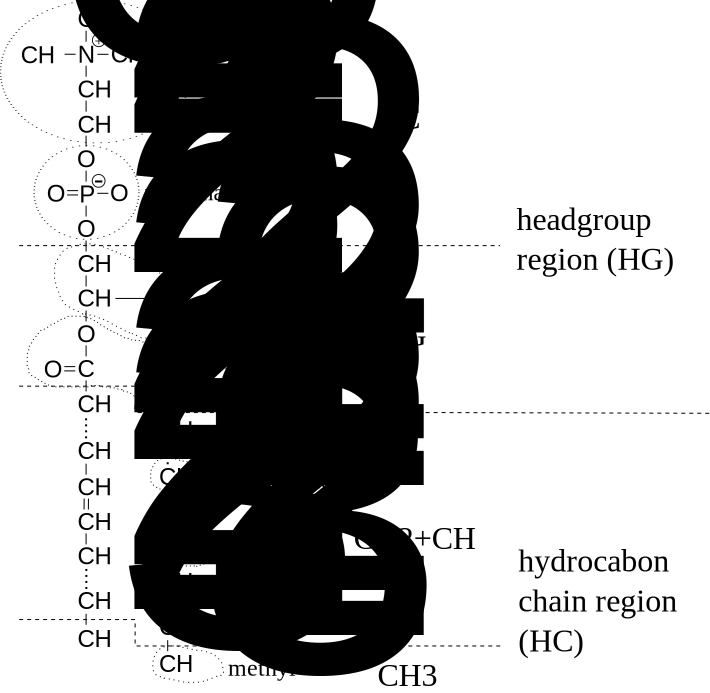
\includegraphics[width=0.9\textwidth]{figures/Tat/dopc_schematic.pdf}
  \caption{Schematic of DOPC showing each lipid component. The dash lines 
           show where the lipid is divided into different components. 
           The lipid headgroup
           is divided into two components, phophate-choline (PC) and carbonyl-glycerol (CG). 
           The hydrocarbon chain region is also divided
           into two components, methylene+methine (CH$_2$+CH) and terminal methyl groups (CH$_3$).}
  \label{fig:dopc_schematic}
\end{figure}

\subsubsection{Functional forms}
Our model for the electron density profile (EDP)
of Tat/lipid bilayer system consists of five structural subgroups: PC, CG,
CH$_2$+CH, CH$_3$, and Tat (see Fig.~\ref{fig:DOPC_EDP}).
The volume probability distributions of components PC, CG, CH$_3$, and Tat 
are described by Gaussian functions,
\begin{equation}
  P_i(z)=\frac{c_i}{\sqrt{2\pi}}\pars{
    \exp\braces{-\frac{(z+z_i)^2}{2\sigma_i^2}}
	+ \exp\braces{-\frac{z-z_i)^2}{2\sigma_i^2}}
  },
\end{equation}
where $c_i$ is an integrated area underneath the curve and the two parts of the 
expression describe the two bilayer leaflets. 

\begin{figure}[htbp]
  \centering
  \includegraphics[width=0.9\textwidth]{figures/Tat/SDP_Results/EDP/DOPC_Tat_model_EDP}
  \caption{A model electron density profile for DOPC with Tat.}
  \label{fig:DOPC_EDP}
\end{figure}

The hydrocarbon chain region (HC) is represented by error functions,
\begin{equation}
  \PHC(z) = \frac{1}{2}\bracks{
    \mathrm{erf}(z,-\z{HC},\sigmaHC) - \mathrm{erf}(z,\z{HC},\sigmaHC)
  },
\end{equation}
where
\begin{equation}
  \mathrm{erf}(z,z_i,\sigma_i)=\frac{2}{\sqrt{\pi}}
    \int_0^{\frac{z-z_i}{\sqrt{2\sigma}}} \dx e^{-x^2}.
\end{equation}
The volume probability distribution for the methylene and methine group
combination can then be expressed as
\begin{equation}
  \PCHtwoCH(z) = \PHC(z)-\PCHthree(z).
  \label{eq:modelA}
\end{equation}
This definition enforces the total probability $\PHC$ in the hydrocarbon
chain region to equal one, which in turn means that placement of Tat in the  
chain region is prohibited. We call the model defined by Eq.~(\ref{eq:modelA})
model A. To allow Tat to be placed inside the hydrocarbon
chain region, we also consider an alternative definition,
\begin{equation}
  \PCHtwoCH(z) = \PHC(z)-\PCHthree(z) - \PTat(z),
\end{equation}
where the volume probability of CH$_2$+CH combined component is reduced by 
the Tat volume probability distribution. We call this model B.
The spatial conservation requires the water volume probability distribution 
to be
\begin{equation}
  \PW(z) = 1-\PPC(z)-\PCG(z)-\PTat(z)-\PHC(z)
\end{equation}
for model A and
\begin{equation}
  \PW(z) = 1-\PPC(z)-\PCG(z)-\PHC(z)
\end{equation}
for model B. 

Because X-rays measure the contrast between the bilayer and surrounding solvents, 
water, the experimental form factor is compared to the water subtracted model
form factor,
\begin{equation}
  F(q_z) = 2\int_0^{\frac{D}{2}} \dz \pars{
    \sum_i(\rho_i-\rhoW)P_i(z)
  } \cos(q_zz),
\end{equation}
where $i$ = PC, CG, Tat, CH+CH$_2$, and CH$_3$.

%%%%%%%%%%%%%%%%%%%%%%%%%%%%%%%%%%%%%%%%%%%%%%%%%%%%%%%%%%%%%%%%%%%%%%%%%%%%%%%
\subsubsection{Constraints}
The height of the hydrocarbon chain error function is fixed to one by imposing
spatial conservation, whereas the mean position of the terminal methyls is
fixed to $\zCHthree=0$ by symmetry arguments. The total lipid volume
$\VL$ is fixed to the experimentally measured value. 
The headgroup volume $\VHL$ was determined to be 331 \AA$^3$ for 
gel phase phosphatidylcholine (PC) bilayers \cite{Tristram-Nagle02},
and we assume the same volume for the fluid phase PC bilayers.
The volumes of PC and CG components satisfy
\begin{equation}
  \VPC + \VCG = \VHL,
\end{equation}
and the volumes of CH$_3$ and CH$_2$+CH components satisfy
\begin{equation}
  2\left(16\VCHtwoCH + \VCHthree\right) = \VL-\VHL.
\end{equation}
These component volumes constrain the height of the Gaussians as
\begin{align}
  \cPC &= \frac{\VPC}{\AL\sigmaPC} \\
  \cCG &= \frac{\VCG}{\AL\sigmaCG} \\
  \cCHthree &= \frac{2\VCHthree}{\AL\sigmaCHthree} \\
  \cTat &= \frac{\VTat}{\AL\sigmaTat}
\end{align}
where $\AL$ is area per lipid.

The ratio of 
the carbonyl/glycerol volume to the headgroup volume $\VHL$ was
reported to be 0.41 \cite{Braun13}, so we constrain the CG
component volume to 135.7 \AA$^3$ and the PC component volume to 
195.3 \AA$^3$. 

The most detailed structural study on DOPC to date was published 
by Braun \textit{et al.} \cite{Braun13}, 
and many of constraints on our model parameters can be derived
from their study. However, in that work, the authors used the 
SDP model \cite{Kucerka08}, which is specifically tailored for
combined analysis of neutron and X-ray form factors. 
Therefore, we need to convert their structural results to the 
corresponding parameters in our simpler model. For example, 
from the reported values of the ratio of the volumes of the chain terminal
methyl (CH$_3$) to the chain methylenes (CH$_2$) and the ratio of 
the volumes of the chain methines (CH) to the chain methylenes, we can
calculate the ratio $\rCHthree$ of the volumes of CH$_3$ to the CH$_2$ and
CH combined component.  
Furthermore, the study by Braun \textit{et al.} was at 30 \textcelsius\
while our study was at 37 \textcelsius, so our
measured volume of DOPC was slightly higher.

At 30 \textcelsius, the volume of DOPC was reported to be 1303 \AA$^3$, 
so the volume of hydrocarbon chain region at the same temperature is 
$1303 - 331 = 972$ \AA$^3$. The ratio $r$ of the volumes
of the chain terminal methyl (CH$_3$) to the chain methylenes (CH$_2$) was 
reported to be 1.95, and the ratio $r_{12}$ of the volumes of the chain
methines (CH) to the chain methylenes 0.91 at 30 \textcelsius. 
Because there are 14 CH$_2$ groups,
2 CH groups, and 1 CH$_3$ group in each DOPC hydrocarbon chain, we have
$2\times(14\VCHtwo+2\VCH+\VCHthree)=972$ \AA$^3$. 
Using $r=\VCHthree/\VCHtwo=1.95$ 
and $r_{12}=\VCH/\VCHtwo=0.91$, we get $\VCHtwo=27.3$ \AA$^3$, 
$\VCH=24.9$ \AA$^3$, and $\VCHthree=53.3$ \AA$^3$. 
These calculated volumes lead to $\VCHthree/\VCHtwoCH=1.97$  for 30 \textcelsius. 

At 37 \textcelsius, the volume of DOPC was measured to be 1313.5 \AA$^3$, so
we have $2\times(16\VCHtwoCH+\VCHthree)=1313.5-331$. Assuming that the ratio 
$\VCHthree/\VCHtwoCH$ at 37 \textcelsius\ is the same as that at 30 \textcelsius\ 
gives $\VCHtwoCH=27.3$ \AA$^3$ and $\VCHthree=53.9$ \AA$^3$. We constrain
the components for the hydrocarbon chain region in our model 
to these calculated values.

\begin{table}[htbp]
  \centering
  \begin{tabular}{ccc}
    \hline
    lipid & number of electrons & volume (\AA$^3$) \\
    \hline
    DOPC & 434 & 1313.5 \\
    DOPE & 410 & 1212.3 \\
    DOPC:DOPE (3:1) & 428 & 1288.2 \\
    \hline
  \end{tabular}
  \caption{Number of electrons per lipid and volume per lipid.}
  \label{tb:electron_volume}
\end{table}

\begin{table}[htbp]
  \centering
  \begin{tabular}{cccc}
    \hline
    component & $n^e_i$ & $V_i$ (\AA$^3$) & $\rho_i$ (e/\AA$^3$) \\
    \hline 
    PC & 97 & 195.3 & 0.497 \\  
    PE & 73 & 94.1  & 0.776 \\
    PC:PE (3:1) & 91 & 170 & 0.535 \\
    CG & 67 & 135.7 & 0.494 \\  
    CH$_2$+CH & 7.875 & 27.3 & 0.288 \\
    CH$_3$ & 9 & 53.9 & 0.167 \\
    \hline
  \end{tabular}
  \caption{Some structural parameters for each component. 
  $n^e_i$ is the number of electrons and
  $\rho_i$ is the average electron density.
  }
  \label{tb:component}
\end{table}

\begin{table}[htbp]
  \centering
  \begin{tabular}{c c c}
    \hline
    number of electrons & 838 \\ 
    volume (\AA$^3$) & 1877 \\
    $\rho_\textrm{Tat}$ (e/\AA$^3$) & 0.446 \\
    \hline
  \end{tabular}
  \quad
  \begin{tabular}{ ccc }
    \hline
    mole fraction ($\xTat$) & $n^e_\textrm{Tat}$ & $\VTat$ (\AA$^3$) \\    
    \hline
    0.016 & 13.6 & 30.5 \\
    0.034 & 29.5 & 66.1 \\
    0.059 & 53.0 & 118.8 \\
    \hline
  \end{tabular}
  \caption{Tat basic structural parameters. The notations are the same
  as in Table~\ref{tb:component}. $\xTat$ = Tat/(Tat+Lipid).}
  \label{tb:Tat_basic_params}
\end{table}

%\begin{table}[htbp]
%  \centering
%  \begin{tabular}{c c c c c c c c}
%    \hline
%     & DOPC & \multicolumn{2}{c|}{62:1} & \multicolumn{2}{c|}{28:1} & \multicolumn{2}{c|}{16:1} \\
%    \cline{3-8}
%     & & A & B & A & B & A & B \\
%    \hline
%    $\VL$ & 1314 & 1344 & 1344 & 1380 & 1380 & 1432 & 1432 \\    
%    $\VHL$ & 331 & 362 & 331 & 397 & 331 & 450 & 331 \\  
%    $\VTat$ & 0 & 30.5 & 30.5 & 66.1 & 66.1 & 119 & 119 \\  
%    $\RPC$ & 0.59 & 0.54 & 0.59 & 0.49 & 0.59 & 0.43 & 0.59 \\
%    $\RCG$ & 0.41 & 0.38 & 0.41 & 0.34 & 0.41 & 0.30 & 0.41 \\
%    $\RTat$ & 0   & 0.08 & 0    & 0.17 & 0    & 0.27 & 0 \\ 
%    $r_{12}$ & 0 & 0 & 0.558 & 0 & 1.21 & 0 & 2.17 \\
%    $r$ & 1.97 & 1.97 & 1.97 & 1.97 & 1.97 & 1.97 & 1.97 \\ 
%    \hline
%  \end{tabular}
%  \caption{Volumetric constraints. A and B refer to two different models 
%  described in the text.}
%  \label{tb:model_constraints}
%\end{table}
%------------------------------------------------------------------------------

%%%%%%%%%%%%%%%%%%%%%%%%%%%%%%%%%%%%%%%%%%%%%%%%%%%%%%%%%%%%%%%%%%%%%%%%%%%%%%%
\subsubsection{Fits with Lower Bounds}
Non-linear least squared fits with upper and lower bounds for the model
parameters are implemented using an internal-external parameter transformation
method. This method is described in MINUIT User's Guide, section 1.3 
\cite{minuit2}. This section briefly describes the method. The details
can be found in the MINUIT website \cite{minuit}.

Basically, instead of a model parameter, which is also called the external variable, 
the minimization procedure varies a related variable called the internal variable.
This internal variable can take any values between $-\infty$ to $+\infty$. 
At every $\chi^2$ calculation, the internal variable is transformed to 
the external variable, which can take values only between the lower and 
upper bounds ($a$ and $b$). This non-linear transformation allows an existing minimization
algorithm that was developed for fits with no bounds to work for fits with bounds.
This point was important because it allowed us to implement bound fits in
the model fitting program called the SDP program, 
fully developed by Dr. Norbert Kucerka, without too many additional changes.
Downsides of the transformation method include turning a linear problem into
a non-linear one and some computational overhead, neither of which is particularly
problematic in this study. 

For variables with both lower and upper bounds 
($a$ and $b$, respectively), the transformation between the internal and
external variables is
\begin{align}
  P_\textrm{int} &= \arcsin \pars{2\frac{P_\textrm{ext}-a}{b-a}-1}  \\
  P_\textrm{ext} &= a + \frac{b-a}{2}(\sin P_\textrm{int}+1).
\end{align}
For variables with a lower bound $a$ only, the transformation is
\begin{align}
  P_\textrm{int} &= \sqrt{(P_\textrm{ext}-a+1)^2 - 1} \\
  P_\textrm{ext} &= a - 1 + \sqrt{P_\textrm{int}^2+1}, 
\end{align}
and for variables with an upper bound $b$ only,
\begin{align}
  P_\textrm{int} &= \sqrt{(b-P_\textrm{ext}+1)^2 - 1} \\
  P_\textrm{ext} &= b + 1 - \sqrt{P_\textrm{int}^2+1}.
\end{align}

%%%%%%%%%%%%%%%%%%%%%%%%%%%%%%%%%%%%%%%%%%%%%%%%%%%%%%%%%%%%%%%%%%%%%%%%%%%%%%%
\subsection{Molecular Dynamics Simulation}\label{sim_methods}
This section describes the MD simulations performed by Dr. Kun Huang, who was
a graduate student of Prof. Angel Garcia at Rensselaer Polytechnic Institute.

Systems with different DOPC/Tat mole ratios (128:0, 128:2 and 128:4, corresponding to
0, 0.015 and 0.030 mole fractions) were simulated atomistically using the Gromacs 4.6.1
package \cite{Hess08}. 
DOPC was modeled by the Slipid force field 
\cite{Jambeck12_JPCB,Jambeck12_JCTC} 
and HIV Tat was modeled by Amber 99SB \cite{Hornak06}. 
Tip3p water was used \cite{Jorgensen83}. The number of Tats was divided equally on
each side of the bilayer to mimic experimental conditions. All systems were simulated at 310 K
with a constant area in the $x$-$y$ plane and 1 atm constant pressure in the $z$ direction. Each
system was simulated for 100 ns and the last 50 ns was used as the production run.
At each DOPC/Tat mole ratio, we studied systems with three different area/lipid ($\AL$).
For the DOPC system, we fixed $\AL$ = 68, 70, 72 \AA$^2$; 
DOPC/Tat (128:2), we fixed the $\AL$ = 72, 74, 76 \AA$^2$; 
DOPC/Tat (128:4), we fixed the $\AL$ = 72, 74, 76 \AA$^2$. 
These values were based on the analysis of experimentally obtained form 
factors, which is discussed in Sec.~\ref{sec:SDP_results}.
For each DOPC/Tat system at fixed $\AL$, 
we then conducted seven independent simulations with the center of mass (COM) of
each Tat constrained at different bilayer depths from the bilayer center 
(18, 16, 14, 12, 10, 8 and 5 \AA). 
In total, 45 independent simulations were conducted. 
The goal of constrained simulations is to find the best match between 
experimental and MD simulation form factors. Comparison to
the X-ray form factors was performed using the SIMtoEXP software 
written by Dr. Norbert Kucerka \cite{Kucerka10}. 

All simulations were conducted with a 2 fs time integration step. SETTLE \cite{Miyamoto92} was used
to constrain water molecules and LINCS \cite{Hess97} was used to constrain all other bond lengths in the
system. VdW interactions were truncated at 1.4 nm with a twin-range cutoff scheme and a
dispersion correction was applied to both energy and pressure. Electrostatics interactions were
treated with the particle-mesh Ewald (PME) method \cite{Darden93}. The direct term for electrostatics was
evaluated within 1.0 nm cutoff and the Fourier term was evaluated with a 0.12 nm grid spacing
and a 4th order interpolation. Each system was simulated at 310 K using the V-rescale
algorithm \cite{Bussi07} with a 0.2 ps time coupling constant. The semi-isotropic parrinello-rahman barostat
\cite{Parrinello81} was used to couple the system at 1 atm in the z direction with a 5 ps time coupling constant,
while the projected area at the x-y plane was fixed by setting the system compressibility to 0.
We inserted the Tats into the system by initially turning off all interactions between Tats and the
rest of the system, with Tats constrained at different depths. Then we slowly turned on the
interactions to normal strength through thermodynamics integrations. We used umbrella
potentials to constrain Tats at desired depths with a force constant of 3000 kJ/mol/nm$^2$.

The center of mass (COM) distance between each peptide and the bilayer was 
constrained by an umbrella potential with a force constant $k$ of 3000 kJ/mol/nm$^2$. 
Essentially, this potential acts as a spring, 
where its potential energy depends on the deviation of the distance 
between the center of mass of Tat and DOPC from a prefered value, $z_0$,
\begin{equation*}
  U(z_1^{\textrm{Tat}},\ldots,z_1^{\textrm{DOPC}},\ldots) = 
  -\frac{1}{2} k 
  \pars{z_{\textrm{cm}}^{\textrm{Tat}} - z_{\textrm{cm}}^{\textrm{DOPC}} - z_0}^2.
\end{equation*}
Then, $-\partial U/\partial z_i$ is the external force acting 
on atom, $i$. 

%%%%%%%%%%%%%%%%%%%%%%%%%%%%%%%%%%%%%%%%%%%%%%%%%%%%%%%%%%%%%%%%%%%%%%%%%%%%%%%
\newpage
\section{Analysis of Molecular Dynamics Simulation Data}
\subsection{SIMtoEXP program}\label{sec:SIMtoEXP}
This section briefly describes the SIMtoEXP program
developed by Dr. Norbert Kucerka \cite{Kucerka10}.
Essentially, for each snapshot, positional distribution of each atom
averaged over the $xy$ plane is calculated. Then, the distribution is
averaged over snapshots. The product of this distribution and the average
electron density gives the electron density profile of the atom. The sum 
over all the atoms provide the total electron density profile. This total
electron density profile minus the average electron density of water
is Fourier transformed to provide the X-ray form factor.
\begin{equation}
  F^\textrm{sim}(q_z) = \int_0^\infty\dz (\rho(z)-\rhoW)\cos (q_zz).
\end{equation}
Electron density profiles were symmetrized and then
X-ray form factors were calculated with $\rhoW$ = 0.326 e/\AA$^3$,
which was the average electron density of water molecules in the MD simulations.
Because $\rho(z)$ is equal to $\rhoW$ outside the bilayer, the upper 
integration limit takes on a finite value. 

Because the experimental form factor is on arbitrary units, it is 
scaled by a single constant $a$ to produce the best fit to the simulated
form factor through a linear least squared fit that minimizes the 
following goodness of fit
\begin{equation}
  \chi^2 = \sum_i \left(\frac{1}{\sigma_i}\pars{
    a|F^\textrm{exp}_i| - |F^\textrm{sim}(q_{z,i})|
  }\right)^2
\end{equation}
where $\sigma_i$ is the input experimental uncertainties and $F_i^\textrm{exp}$
is the experimental form factor measured at $q_z = q_{z,i}$.
The SIMtoEXP program does not scale the input uncertainties, so
the relative errors ($\sigma_i$/$|F_i^\textrm{exp}|$) depend on the value of
the overall scaling factor $a$. Consequently, the $\chi^2$ values calculated by 
the program had to be multiplied by 1/$a^2$. 
These corrected $\chi^2$ are reported in this chapter.

%%%%%%%%%%%%%%%%%%%%%%%%%%%%%%%%%%%%%%%%%%%%%%%%%%%%%%%%%%%%%%%%%%%%%%%%%%%%%%%
\subsection{Local Thinning of Membranes}\label{sec:local_thinning}
My contribution to the MD simulations was to help analyze the results.

The SIMtoEXP program only gives the average quantities for each leaflet. 
While our X-ray data are sensitive to the bilayer average electron density,
local information of Tat-bilayer interactions can be obtained from MD simulations.
In this section, we discuss a method to extract a local membrane thickness
around the Tat peptides from the MD simulation trajectories. 

One of the expected effects of Tat interacting with a bilayer is 
compression of the lipid bilayer along the $z$-direction. It is 
reasonable to assume that this compression is greater near Tat and
weaker far from Tat.
If this is the case, the distance between phosphorus atoms in opposite
leaflets near Tat should be different from the distance between
phosphorus atoms away from Tat.  
For a small Tat concentration, $D_\textrm{phos-phos}$ is the same as that of 
pure DOPC if the distance from all Tats is large enough.  
For our experimental concentrations, the thinning effect may extend throughout 
the bilayer because the lateral effect of Tat might have a larger lateral decay 
length than the distance between Tats. Whether that is the case or not, we 
expect that the thickness near the Tats is smaller than the average thickness,
so $D_\textrm{phos-phos}'$ is what we want to measure. 

\begin{figure}[htbp]
  \centering
  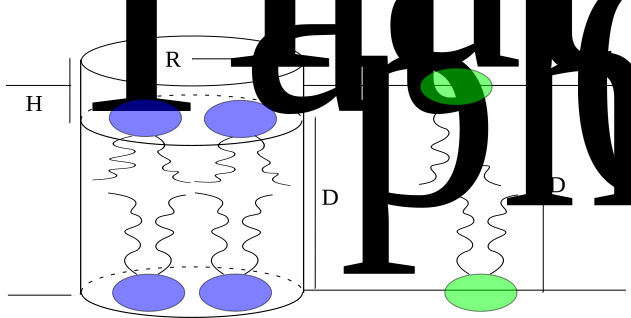
\includegraphics[scale=0.7]{./figures/Tat/cylinder_model}
  \caption{Our simple model to extract the local bilayer thickness from 
  simulation trajectories. Tat is modeled as a cylinder with its height $\HTat$ 
  and radius $\RTat$. The local thickness is defined as $D_\textrm{phos-phos}'$. 
  The thickness of the unperturbed DOPC bilayer is $D_\textrm{phos-phos}$. 
  Blue highlighted lipids fall within the imaginary cylinder extended from
  the Tat. Unperturbed lipids are highlighted in green.}
  \label{fig:cylinder_model}
\end{figure}
 
First, let us define what we mean by lipids close to Tat.  
As in Fig.~\ref{fig:cylinder_model}, we imagine a cylinder around Tat and 
find all the phosphorus atoms within it. 
Approximating Tat as a cylinder 
with its height given by the FWHM of its electron density distribution, 
its radius $\RTat$ = 9 \AA\ comes from the experimentally determined volume $\VTat$ = 1876 \AA$^3$ and 
$\HTat$ = 7.6 \AA\ measured from one of the simulations (see Sec.~\ref{sec:sim_results}). 
Let us define the lateral center of the cylinder as the center of mass of each
Tat. Then we define $D_\textrm{phos-phos}'$ using only those lipids whose 
phosphorus atoms lie within these 9 \AA\ cylinders around the 
Tats. 
Then $D_\textrm{phos-phos} = \zphos^+ - \zphos^-$ where $\zphos^+$ and $\zphos^-$ 
are the average $z$ of the $n_1$ ($n_2$) lipids in the upper and lower monolayer, respectively.  

The algorithm for doing the above was straightforward.  
For each time frame, the positions ($x_i$ ,$y_i$, $z_i$) of each Tat, $i$, are 
listed.   
We chose phosphorus atoms whose ($x$, $y$) lateral position lied within 
9 \AA\ of any one of the Tat's lateral position. Then, $z$ positions
of the chosen phosphorus atoms were placed in a list. 
Then, $\zphos$ were calculated from the list. 
We averaged over many snapshots to gain better statistics. 

%%%%%%%%%%%%%%%%%%%%%%%%%%%%%%%%%%%%%%%%%%%%%%%%%%%%%%%%%%%%%%%%%%%%%%%%%%%%%%%
\subsection{Lateral Decay Length of Membrane Thinning}\label{sec:lateral_decay}
This section describes a method to measure the lateral decay length
of membrane thinning due to Tat-lipid interactions. 
As in the previous section, Tat is modeled here as a cylinder with 
its radius equal to $R_1$, height $\HTat$,
and volume $\VTat$ such that $R_1=\sqrt{\VTat/(\pi \HTat)}$. 
Let $h(r)$ represent the phosphorus height profile
of a leaflet as in Fig.~\ref{fig:linear_model}. The two leaflets are assumed to be decoupled.
In our model, lipids are separated into three regions: 
suppressed, boundary, and unperturbed region . 
The suppressed region extends from $r=0$ to $R_1$ and is directly beneath 
(above) Tat in the top (bottom) leaflet. In this region, lipids are uniformly 
compressed by Tat toward the 
center of the bilayer, so that $h(r)$ is a constant equal to $\zphos$. 
From $r=R_1$ to $R_2$ is the boundary region, where $h(r)$ is assumed to 
linearly increase with the lateral distance $r$. The lateral decay length
of membrane thinning is given by $R_2-R_1$. 
In the unperturbed region ($r>R_3$), lipids do not interact with 
Tat, behaving identically to DOPC, so the phosphorus position is the same as that of 
DOPC. A continuous $h(r)$ that 
satisfies the above criteria is
\begin{equation}
  h(r) = \left\{ 
  \begin{array}{lcr}
    \zphos   & \text{if} & 0   \leq r < R_1 \\
    mr+b     & \text{if} & R_1 \leq r < R_2 \\
    \zphos^0 & \text{if} & R_2 \leq r < R_3 
  \end{array}\right.  
\end{equation}     
with $m=(\zphos-\zphos^0)/(R_1-R_2)$ and $b=(\zphos^0R_1-\zphos R_2)/(R_1-R_2)$. 
Approximating the simulation box as a cylinder gives 
$R_3=\sqrt{N\AL/\pi}$, where $N$ is the number of lipids in a leaflet. 
$\zphos$ can be measured directly from simulation trajectories.
$\zphos^0$ is a half of the average phosphorus-phosphorus distance 
in a DOPC simulation,
which can be easily obtained from the SIMtoEXP program. 
The average height profile over
the monolayer, $\langle h(r) \rangle$, can be also obtained from the program 
in the same manner. 
The only unknown is $R_2$.

\begin{figure}[htbp]
  \centering
  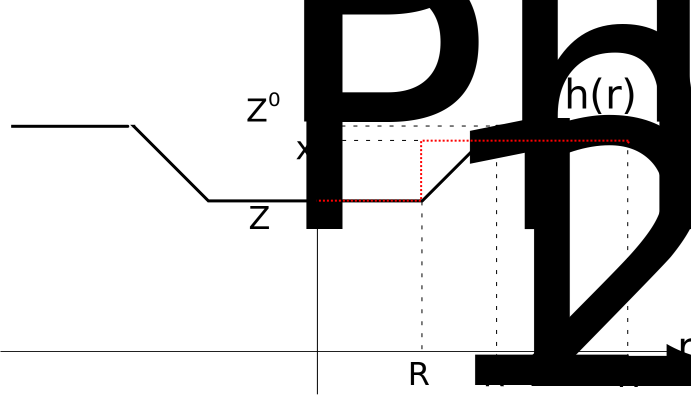
\includegraphics[width=0.7\textwidth]{./figures/Tat/linear_model}
  \caption{Simple model of the lateral decay of the membrane thickness 
  perturbation due to Tat.}
  \label{fig:linear_model}
\end{figure}

Let us calculate $\langle h(r) \rangle$. In cylindrical coodinates, 
\begin{equation}
  \langle h(r) \rangle 
  = \frac{1}{\pi R_3^2} \int_0^{2\pi}d\phi \int_0^{R_3}\dr rh(r)
\end{equation}
The $\phi$ integration is trivial. The $r$ integration is
\begin{align}
  & \int_0^{R_3}\dr rh(r) \nonumber\\
  &= \int_0^{R_1}\dr \zphos r + \int_{R_1}^{R_2}\dr (mr+b)r + \int_{R_2}^{R_3}\dr \zphos^0r \nonumber\\
  &= \frac{1}{2}\left[\zphos R_1^2+\zphos^0(R_3^2-R_2^2)\right] + 
     \frac{1}{3}m\left(R_2^3-R_1^3\right) + 
     \frac{1}{2}b\left(R_2^2-R_1^2\right) \nonumber\\        
  &= \frac{1}{2}\left[\zphos R_1^2+\zphos^0(R_3^2-R_2^2)\right] +
     \frac{1}{3}\left(\zphos^0-\zphos\right)\left(R_2^2+R_1R_2+R_1^2\right) \nonumber\\
  &  + \frac{1}{2}\left(\zphos R_2-\zphos^0 R_1\right)\left(R_1+R_2\right) \label{eq:r_integ}
\end{align}
Using Eq.~(\ref{eq:r_integ}), we get 
\begin{equation}
  \langle h(r) \rangle 
  = \frac{\left(\zphos-\zphos^0\right)\left(R_1^2+R_1R_2+R_2^2\right)+3\zphos^0R_3^2}{3R_3^2}
  \label{eq:quadR2}
\end{equation}
Eq.~\ref{eq:quadR2} is a quadratic equation in terms of $R_2$. 
Solving for $R_2$ gives
\begin{equation}
  R_2 = \frac{-R_1+\sqrt{R_1^2+4C}}{2} 
\end{equation}
with
\begin{equation}
  C = \frac{3R_3^2\left(\zphos^0-\langle h(r)\rangle\right)}{\zphos^0-\zphos} - R_1^2
\end{equation}

%%%%%%%%%%%%%%%%%%%%%%%%%%%%%%%%%%%%%%%%%%%%%%%%%%%%%%%%%%%%%%%%%%%%%%%%%%%%%%%
\section{Results}
\subsection{Bending and Bulk Modulus}\label{sec:Kc_results}
(Under construction)
Show X-ray data. Show fitting boxes. Show the Kc values.
Also, show the resultant form factors, which qualitatively show the membrane thinning.
Also describe how I got error bars.

Fig.~\ref{fig:figure1} shows the scattering intensity pattern from DOPC/DOPE (1:1) with mole 
fraction $\xTat=0.034$. The diffuse lobes are due to equilibrium fluctuations that occur 
in these fully hydrated, oriented lipid/peptide samples. The intensity $I(\mathbf{q})$ in the diffuse 
patterns provide the
absolute values of the form factors $F(q_z)$, which are the Fourier transforms 
of the electron density
profile, through the relation $I(\mathbf{q})=S(\mathbf{q})|F(q_z)|^2/q_z$, 
where $\mathbf{q}=(q_r,q_z)$, $S(q)$ is 
the structure
interference factor, and $q_z^{−1}$ is the usual LAXS approximation to the 
Lorentz factor \cite{Kucerka05_BPJ,Kucerka06,Kucerka05_JMB}.
The first step in the analysis takes advantage of the $q_r$ dependence of the 
scattering to obtain the
bending modulus $K_c$ with results shown in Fig.~\ref{fig:figure2}. 
As positively charged Tat concentration was increased, 
the lamellar repeat spacing $D$ generally increased in neutral lipid 
bilayers and decreased in negatively charged bilayers, consistent with changes in 
electrostatic repulsive interactions. 
With few exceptions, the water space between bilayers exceeded 20 \AA.

\begin{figure}[htbp]
  \centering
  \includegraphics[width=0.8\textwidth]{figures/Tat/figure2}
  \caption{Bilayer bending modulus, $K_c$, vs. Tat mole fraction $\xTat$. 
  $D$-spacings for DOPC/Tat mixtures varied from 64 to 68 \AA, 
  for DOPC/DOPE/Tat mixtures from 64 to 69 \AA, 
  for DOPC/DOPS/Tat (3:1) mixtures from 57 \AA to > 100 \AA (pure DOPS was unbound), 
  and for nuclear mimic/Tat mixtures from unbound (nuclear mimic) to 64 \AA. 
  Estimated uncertainty in all values is about $\pm$ 2.}
  \label{fig:figure2}
\end{figure}

The analysis that obtains $K_c$ also obtains the structure factor $S(\mathbf{q})$ 
and then the unsigned form factors $|F(q_z)|$ are obtained from the intensity $I(\mathbf{q})$ by division. 
Results for five different membrane mimics are shown in Fig.~\ref{fig:figure3}. 
Vertical lines indicate the “zero” position between the lobes of diffuse data 
where $F(q_z)$ change sign. In every sample, the zero positions shift to larger
$q_z$, indicating a thinning of the membranes.

\begin{figure}[htbp]
  \centering
  \includegraphics[width=0.45\textwidth]{figures/Tat/figure3a}
  \includegraphics[width=0.43\textwidth]{figures/Tat/figure3b}
  \includegraphics[width=0.55\textwidth]{figures/Tat/figure3c}
  \includegraphics[width=0.19\textwidth]{figures/Tat/figure3d}
  \includegraphics[width=0.175\textwidth]{figures/Tat/figure3e}
  \caption{Form factors of lipid mixtures (arbitrarily scaled and vertically displaced) with
  increasing Tat mole fractions $\xTat$ indicated on figure legends. Lipid mixtures: A. DOPC
  B. DOPC/DOPE (3:1) C. DOPC/DOPE (1:1) D. DOPC/DOPS (3:1) E. Nuclear mimic. The
  entire $q_z$ range is shown in C, while others show partial ranges. Solid vertical lines indicate the
  $q_z$ values where the form factors equal zero between the lobes of diffuse data.}
  \label{fig:figure3}
\end{figure}

%%%%%%%%%%%%%%%%%%%%%%%%%%%%%%%%%%%%%%%%%%%%%%%%%%%%%%%%%%%%%%%%%%%%%%%%%%%%%%%
\subsection{Volume results}\label{sec:volume_results}
Experimental and simulated volumes are given in Table~\ref{tb:volumes}. The simulated volume was
obtained using the volume app in the SIMtoEXP program. The experimental Tat volume was
calculated from the measured density assuming that the lipid volume was the same as with no
Tat. In general, there may be an interaction volume between the peptide and the lipid membrane
as previously reported for bacteriorhodopsin \cite{Tristram-Nagle86}. As lipid was present in excess to Tat, the
partial molecular volume of the lipid should be the same as with no Tat, so this way of
calculating includes all the interaction volume in $\VTat$. Comparison of $\VTat$ in water with the
result for 5:1 Lipid:Tat suggests that the interaction volume may be negative, consistent with a
net attractive interaction with lipid. Understandably, values of $\VTat$ were unreliable for small
mole ratios of Tat:Lipid. Therefore we used simple additivity for those mimics not shown in
Table~\ref{tb:volumes} for the volumes used in the electron density profile modeling. 
All volumes obtained from the Gromacs MD
simulations were somewhat smaller than the measured volumes, but it supports the Tat volume
being closer to 1877 \AA$^3$ than the outlying values obtained experimentally at small Tat
concentrations. The measured volume was in a good agreement with the 
value calculated from a peptide calculator website \cite{peptide_calc}, which
gave 1888 \AA$^3$. 

%------------------------------------------------------------------------------
%\begin{table}[htbp]
%  \centering
%  \begin{tabular}{c c}
%    $\rho_{sol}$ & 0.994180 $\mathrm{g/cm^3}$\\
%    $\rho_w$ & 0.993325 $\mathrm{g/cm^3}$\\
%    $m_w$ & 1212.6 mg \\
%    $m_T$ & 3.73 mg \\ 
%  \end{tabular}
%  \caption{Measured Quantities in }
%  \label{tb:values}
%\end{table}

\begin{table}[htbp]
  \centering
  Experiments\\
  \begin{tabular}{cccc}
    \hline
    Tat in: & $V_\textrm{lipid}$ (\AA$^3$) & Lipid:Tat & $\VTat$ (\AA$^3$) \\
    \hline
    water & & 1877 \\
    DOPC:DOPE (3:1) & 1288 & 5:1 & 1822 \\
    DOPC & 1314 & 39.6:1 & 676 \\
    DOPC:DOPS (3:1) & 1298 & 39.6:1 & 2613 \\
    \hline 
  \end{tabular}
  \quad
  \begin{tabular}{cccc}
    & & & \\
    \multicolumn{4}{c}{Simulations} \\ 
    \hline
    Tat in: & $V_\textrm{lipid}$ (\AA$^3$) & Lipid:Tat & $\VTat$ (\AA$^3$) \\
    \hline
    DOPC & 1283 & 128:2 & 1694 \\
    DOPC & 1294 & 128.4 & 1699 \\
    \hline
  \end{tabular}
  \caption{Volume results at 37 \textcelsius}
  \label{tb:volumes}
\end{table}

%%%%%%%%%%%%%%%%%%%%%%%%%%%%%%%%%%%%%%%%%%%%%%%%%%%%%%%%%%%%%%%%%%%%%%%%%%%%%%%
\subsection{Electron Density Profile Modeling}\label{sec:SDP_results}
(Under construction)
Using the model described in section \ref{sec:SDP_method}, 
we fitted our measured X-ray form factors. In all fits,
the positions of component groups were free parameters, but we 
assumed that the lipid headgroup is somewhat rigid so that it cannot compress
or expand. This assumption led to fixing the distance
$\zPC-\zCG$ between the PC and CG components as well
as the distance $\zCG-\zHC$ between the CG component and the Gibbs dividing
surface for the hydrocarbon chains. 
We also constrained the width of Tat 
Gaussian. We fitted with three different values of widths,
2.5, 3.0, and 3.5, to study the range of variation due to the Tat width. 
The choice was made based on MD simulation results. (Check this again)
We constrained the Tat width 
because we found that this parameter tended to become very small
when it was free. This tendency to a unphysically small value was due to 
lack of higher $q_z$ data points. A very narrow feature in an electron density profile
led to large magnitude of the form factor at larger $q_z$. Because data 
points at larger $q_z$ were not available, this narrow feature did not get penalized. 
In wide angle X-ray scattering, which probes much larger $q_z$ than LAXS does,
we did not observe much diffuse scattering for $q_z > 1.0$ \AA$^{-1}$ (data not shown).
Also, from a stereochemical point of view, a peptide width cannot be too small.
These arguments allowed us to disregard the best fits with a too small value
of $\sigmaTat$ and led to fixing the Tat width.

Figure~\ref{fig:DOPC_Tat_XFF1} shows the results for DOPC with Tat. 
As shown, the fits were generally very good.  
Table~\ref{tb:DOPC_fit_results} shows the best fit parameters for DOPC bilayers.
It is clear that the area per lipid $\AL$ increased as the Tat concentration was
increased. An increase in $\AL$ implies thinning of the bilayer which is an 
incompressible membrane. The results for DOPC:DOPE (3:1) are shown in 
Fig.~\ref{fig:DOPCDOPE3to1_Tat_XFF1} and 
Table~\ref{tb:DOPCDOPE3to1_fit_results}, and the results for DOPC:DOPE (1:1) 
in Fig.~\ref{fig:DOPCDOPE1to1_Tat_XFF1} and 
Table~\ref{tb:DOPCDOPE1to1_fit_results}. Figure~\ref{fig:figure6} summarizes
these results. For the results shown in Fig.~\ref{fig:figure6}, a
consistent trend is that Tat moved away from the bilayer center as concentration increased.

\begin{figure}[htbp]
  \centering
  \includegraphics[width=0.45\textwidth,valign=t]{figures/Tat/SDP_Results/XFF/DOPC_XFF1} 
  \includegraphics[width=0.45\textwidth,valign=t]{figures/Tat/SDP_Results/EDP/DOPC_EDP1} 
  \includegraphics[width=0.45\textwidth,valign=t]{figures/Tat/SDP_Results/XFF/DOPC_Tat_62to1_3p0_XFF1}
  \includegraphics[width=0.45\textwidth,valign=t]{figures/Tat/SDP_Results/EDP/DOPC_Tat_62to1_3p0_EDP1} 
  \includegraphics[width=0.45\textwidth,valign=t]{figures/Tat/SDP_Results/XFF/DOPC_Tat_28to1_3p0_XFF1}
  \includegraphics[width=0.45\textwidth,valign=t]{figures/Tat/SDP_Results/EDP/DOPC_Tat_28to1_3p0_EDP1}
  \includegraphics[width=0.45\textwidth,valign=t]{figures/Tat/SDP_Results/XFF/DOPC_Tat_16to1_3p0_XFF1}
  \includegraphics[width=0.45\textwidth,valign=t]{figures/Tat/SDP_Results/EDP/DOPC_Tat_16to1_3p0_EDP1}
  \caption{The best fits to DOPC form factors (left) and the corresponding 
  electron density profiles (right) with $\xTat$ = 0, 0.016, 0.034, 
  and 0.059 (from top to bottom).}
  \label{fig:DOPC_Tat_XFF1}
\end{figure}

\begin{table}[htbp]
  \centering
  \begin{tabular}{ccccccccccc}
    \hline
    $\xTat$ & 0 & 0.016 & 0.016 & 0.016 & 0.034 & 0.034 & 0.034 & 0.059 & 0.059 & 0.059 \\
    \hline
    $\chi^2$ & 2961 & 1554 & 1570 & 1581 & 1563 & 1587 & 1607 & 2342 & 2338 & 2363 \\ 
    $\zPC$ & 18.1 & 18.0 & 17.9 & 17.9 & 17.8 & 17.7 & 17.6 & 17.8 & 17.8 & 17.7 \\
    $\sigmaPC$ & 2.52 & 2.14 & 2.17 & 2.18 & 1.86 & 1.92 & 1.93 & 2.02 & 1.97 & 1.93 \\
    $\zCG$ & 15.0 & 14.9 & 14.8 & 14.8 & 14.7 & 14.6 & 14.5 & 14.7 & 14.7 & 14.6 \\
    $\sigmaCG$ & 3.00 & 2.62 & 2.64 & 2.66 & 2.22 & 2.30 & 2.31 & 2.58 & 2.27 & 2.14 \\
    $\zHC$ & 13.7 & 13.6 & 13.5 & 13.5 & 13.4 & 13.3 & 13.2 & 13.4 & 13.4 & 13.3 \\ 
    $\sigmaHC$ & 3.00 & 2.69 & 2.84 & 2.95 & 2.65 & 2.82 & 3.01 & 2.47 & 2.58 & 2.83 \\
    $\sigmaCHthree$ & 3.20 & 3.19 & 3.22 & 3.24 & 3.37 & 3.43 & 3.47 & 2.70 & 2.70 & 2.74 \\
    $\zTat$ & NA & 12.9 & 13.4 & 14.2 & 13.1 & 13.8 & 14.4 & 15.2 & 15.2 & 15.7 \\
    $\sigmaTat$ & NA & 2.5 & 3.0 & 3.5 & 2.5 & 3.0 & 3.5 & 2.5 & 3.0 & 3.5 \\ 
%    \hline
%    $\VL$ & 1314 & \multicolumn{3}{c|}{1344} & \multicolumn{3}{c|}{1380} & \multicolumn{3}{c|}{1432} \\ 
%    $\VHL$ & 331 & \multicolumn{3}{c|}{362} & \multicolumn{3}{c|}{397} & \multicolumn{3}{c|}{450} \\
%    $\VTat$ & 0 & \multicolumn{3}{c|}{30.5} & \multicolumn{3}{c|}{66.1} & \multicolumn{3}{c|}{118.8} \\
%    $\RPC$ & 0.59 & \multicolumn{3}{c|}{0.54} & \multicolumn{3}{c|}{0.49} & \multicolumn{3}{c|}{0.43} \\
%    $\RCG$ & 0.41 & \multicolumn{3}{c|}{0.38} & \multicolumn{3}{c|}{0.0.34} & \multicolumn{3}{c|}{0.30} \\
%    \hline
%    $\Delta z_1$ & \multicolumn{10}{c|}{3.1} \\
%    $\Delta z_2$ & \multicolumn{10}{c|}{1.3} \\
%    $\rCHthree$ & \multicolumn{10}{c|}{1.97} \\
%    $\rTat$ & \multicolumn{10}{c|}{0} \\
    $\AL$ & 71.5 & 72.4 & 72.5 & 72.7 & 73.6 & 74.0 & 74.4 & 73.6 & 73.5 & 73.9 \\
    \hline
  \end{tabular}
  \caption{Fitting Results for DOPC membranes for the THG (Tat in headgroup) model. $\zPC-\zCG = 3.1$ \AA\
  and $\zCG-\zHC = 1.3$ \AA\ in all fits.}
  \label{tb:DOPC_fit_results}
\end{table}

\begin{figure}[htbp]
  \centering
  \includegraphics[width=0.45\textwidth,valign=t]{figures/Tat/SDP_Results/XFF/DOPCDOPE3to1_XFF1}
  \includegraphics[width=0.45\textwidth,valign=t]{./figures/Tat/SDP_Results/EDP/DOPCDOPE3to1_EDP1}
  \includegraphics[width=0.45\textwidth,valign=t]{figures/Tat/SDP_Results/XFF/DOPCDOPE3to1_Tat_62to1_3p0_XFF1}
  \includegraphics[width=0.45\textwidth,valign=t]{./figures/Tat/SDP_Results/EDP/DOPCDOPE3to1_Tat_62to1_3p0_EDP1}
  \includegraphics[width=0.45\textwidth,valign=t]{figures/Tat/SDP_Results/XFF/DOPCDOPE3to1_Tat_28to1_3p0_XFF1}
  \includegraphics[width=0.45\textwidth,valign=t]{./figures/Tat/SDP_Results/EDP/DOPCDOPE3to1_Tat_28to1_3p0_EDP1}
  \includegraphics[width=0.45\textwidth,valign=t]{figures/Tat/SDP_Results/XFF/DOPCDOPE3to1_Tat_16to1_3p0_XFF1}
  \includegraphics[width=0.45\textwidth,valign=t]{./figures/Tat/SDP_Results/EDP/DOPCDOPE3to1_Tat_16to1_3p0_EDP1}
  \caption{The best fits to DOPC:DOPE (3:1) form factors (left) and the corresponding 
  electron density profiles (right) with $\xTat$ = 0, 0.016, 0.034, 
  and 0.059 (from top to bottom).}
  \label{fig:DOPCDOPE3to1_Tat_XFF1}
\end{figure}

\begin{table}[htbp]
  \centering
  \begin{tabular}{ccccccccccc}
    \hline
    $\xTat$ & 0 & 0.016 & 0.016 & 0.016 & 0.034 & 0.034 & 0.034 & 0.059 & 0.059 & 0.059 \\
    \hline
    $\chi^2$ & 924.5 & 4972 & 4985 & 4994 & 6758 & 6826 & 6863 & 2293 & 2280 & 2296 \\ 
    $\zPC$ & 18.3 & 18.5 & 18.5 & 18.4 & 18.5 & 18.4 & 18.3 & 18.2 & 18.2 & 18.1 \\
    $\sigmaPC$ & 2.66 & 2.23 & 2.26 & 2.27 & 2.25 & 2.31 & 2.34 & 2.31 & 2.19 & 2.11 \\
    $\zCG$ & 15.2 & 15.4 & 15.4 & 15.3 & 15.4 & 15.3 & 15.2 & 15.1 & 15.1 & 15.0 \\
    $\sigmaCG$ & 2.92 & 2.63 & 2.65 & 2.69 & 2.52 & 2.58 & 2.63 & 2.40 & 2.20 & 2.01 \\
    $\zHC$ & 13.9 & 14.1 & 14.1 & 14.0 & 14.1 & 14.0 & 13.9 & 13.8 & 13.8 & 13.7 \\
    $\sigmaHC$ & 2.73 & 2.70 & 2.83 & 2.91 & 2.86 & 2.79 & 2.84 & 2.25 & 2.38 & 2.60 \\
    $\sigmaCHthree$ & 3.24 & 2.94 & 2.97 & 2.98 & 2.87 & 2.90 & 2.91 & 2.63 & 2.61 & 2.65 \\
    $\zTat$ & NA & 13.5 & 14.0 & 15.0 & 14.3 & 14.9 & 16.0 & 16.3 & 16.4 & 16.9 \\
    $\sigmaTat$ & NA & 2.5 & 3.0 & 3.5 & 2.5 & 3.0 & 3.5 & 2.5 & 3.0 & 3.5 \\ 
%    \hline
%    $\VL$ & 1288 & \multicolumn{3}{c|}{1319} & \multicolumn{3}{c|}{1354} & \multicolumn{3}{c|}{1407} \\ 
%    $\VHL$ & 306 & \multicolumn{3}{c|}{336} & \multicolumn{3}{c|}{372} & \multicolumn{3}{c|}{425} \\
%    $\VTat$ & 0 & \multicolumn{3}{c|}{30.5} & \multicolumn{3}{c|}{66.1} & \multicolumn{3}{c|}{118.8} \\
%    $\RPC$ & 0.59 & \multicolumn{3}{c|}{0.54} & \multicolumn{3}{c|}{0.49} & \multicolumn{3}{c|}{0.43} \\
%    $\RCG$ & 0.41 & \multicolumn{3}{c|}{0.38} & \multicolumn{3}{c|}{0.0.34} & \multicolumn{3}{c|}{0.30} \\
%    \hline
%    $\Delta z_1$ & \multicolumn{10}{c|}{3.1} \\
%    $\Delta z_2$ & \multicolumn{10}{c|}{1.3} \\
%    $\rCHthree$ & \multicolumn{10}{c|}{1.97} \\
%    $\rTat$ & \multicolumn{10}{c|}{0} \\
%    \hline
    $\AL$ & 70.9 & 69.8 & 69.9 & 70.1 & 69.5 & 70.0 & 70.6 & 71.3 & 71.4 & 71.7 \\
    \hline
  \end{tabular}
  \caption{Fitting Results for DOPC:DOPE (3:1) membranes for the THG model. $\zPC-\zCG = 3.1$ \AA\
  and $\zCG-\zHC = 1.3$ \AA\ in all fits.}
  \label{tb:DOPCDOPE3to1_fit_results}
\end{table}

\begin{figure}[htbp]
  \centering
  \includegraphics[width=0.45\textwidth,valign=t]{figures/Tat/SDP_Results/XFF/DOPCDOPE1to1_XFF1}
  \includegraphics[width=0.45\textwidth,valign=t]{./figures/Tat/SDP_Results/EDP/DOPCDOPE1to1_EDP1}
  \includegraphics[width=0.45\textwidth,valign=t]{figures/Tat/SDP_Results/XFF/DOPCDOPE1to1_Tat_62to1_3p0_XFF1}
  \includegraphics[width=0.45\textwidth,valign=t]{./figures/Tat/SDP_Results/EDP/DOPCDOPE1to1_Tat_62to1_3p0_EDP1}
  \includegraphics[width=0.45\textwidth,valign=t]{figures/Tat/SDP_Results/XFF/DOPCDOPE1to1_Tat_28to1_3p0_XFF1}
  \includegraphics[width=0.45\textwidth,valign=t]{./figures/Tat/SDP_Results/EDP/DOPCDOPE1to1_Tat_28to1_3p0_EDP1}
  \includegraphics[width=0.45\textwidth,valign=t]{figures/Tat/SDP_Results/XFF/DOPCDOPE1to1_Tat_16to1_3p0_XFF1}
  \includegraphics[width=0.45\textwidth,valign=t]{./figures/Tat/SDP_Results/EDP/DOPCDOPE1to1_Tat_16to1_3p0_EDP1}
  \caption{The best fits to DOPC:DOPE (1:1) form factors (left) and the corresponding 
  electron density profiles (right) with $\xTat$ = 0, 0.016, 0.034, 
  and 0.059 (from top to bottom).}
  \label{fig:DOPCDOPE1to1_Tat_XFF1}
\end{figure}

\begin{table}[htbp]
  \centering
  \begin{tabular}{c c c c c c c c c c c}
    \hline
    $\xTat$ & 0 & 0.016 & 0.016 & 0.016 & 0.034 & 0.034 & 0.034 & 0.059 & 0.059 & 0.059 \\
    \hline
    $\chi^2$ & 2961 & 1554 & 1570 & 1581 & 1563 & 1587 & 1607 & 2342 & 2338 & 2363 \\     
    $\zPC$ & 18.1 & 18.0 & 17.9 & 17.9 & 17.8 & 17.7 & 17.6 & 17.8 & 17.8 & 17.7 \\
    $\sigmaPC$ & 2.52 & 2.14 & 2.17 & 2.18 & 1.86 & 1.92 & 1.93 & 2.02 & 1.97 & 1.93 \\
    $\zCG$ & 15.0 & 14.9 & 14.8 & 14.8 & 14.7 & 14.6 & 14.5 & 14.7 & 14.7 & 14.6 \\
    $\sigmaCG$ & 3.00 & 2.62 & 2.64 & 2.66 & 2.22 & 2.30 & 2.31 & 2.58 & 2.27 & 2.14 \\
    $\zHC$ & 13.7 & 13.6 & 13.5 & 13.5 & 13.4 & 13.3 & 13.2 & 13.4 & 13.4 & 13.3 \\ 
    $\sigmaHC$ & 3.00 & 2.69 & 2.84 & 2.95 & 2.65 & 2.82 & 3.01 & 2.47 & 2.58 & 2.83 \\
    $\sigmaCHthree$ & 3.20 & 3.19 & 3.22 & 3.24 & 3.37 & 3.43 & 3.47 & 2.70 & 2.70 & 2.74 \\
    $\zTat$ & NA & 12.9 & 13.4 & 14.2 & 13.1 & 13.8 & 14.4 & 15.2 & 15.2 & 15.7 \\
    $\sigmaTat$ & NA & 2.5 & 3.0 & 3.5 & 2.5 & 3.0 & 3.5 & 2.5 & 3.0 & 3.5 \\ 
%    \hline
%    $\VL$ & 1314 & \multicolumn{3}{c|}{1344} & \multicolumn{3}{c|}{1380} & \multicolumn{3}{c|}{1432} \\ 
%    $\VHL$ & 331 & \multicolumn{3}{c|}{362} & \multicolumn{3}{c|}{397} & \multicolumn{3}{c|}{450} \\
%    $\VTat$ & 0 & \multicolumn{3}{c|}{30.5} & \multicolumn{3}{c|}{66.1} & \multicolumn{3}{c|}{118.8} \\
%    $\RPC$ & 0.59 & \multicolumn{3}{c|}{0.54} & \multicolumn{3}{c|}{0.49} & \multicolumn{3}{c|}{0.43} \\
%    $\RCG$ & 0.41 & \multicolumn{3}{c|}{0.38} & \multicolumn{3}{c|}{0.0.34} & \multicolumn{3}{c|}{0.30} \\
%    \hline
%    $\Delta z_1$ & \multicolumn{10}{c|}{3.1} \\
%    $\Delta z_2$ & \multicolumn{10}{c|}{1.3} \\
%    $\rCHthree$ & \multicolumn{10}{c|}{1.97} \\
%    $\rTat$ & \multicolumn{10}{c|}{0} \\
%    \hline
    $\AL$ & 71.5 & 72.4 & 72.5 & 72.7 & 73.6 & 74.0 & 74.4 & 73.6 & 73.5 & 73.9 \\
    \hline
  \end{tabular}
  \caption{(Numbers are wrong) Fitting Results for DOPC:DOPE (1:1) membranes for the THG model. $\Delta z_1 = \zPC-\zCG$
  and $\Delta z_2 = \zCG-\zHC$.}
  \label{tb:DOPCDOPE1to1_fit_results}
\end{table}

\begin{figure}
  \centering
  \includegraphics[width=0.5\textwidth]{figures/Tat/figure6}
  \caption{Modeling results for absolute electron density profiles
  and for the Tat location as a function of distance $z$ along the
  bilayer normal. A. DOPC B. DOPC:DOPE (3:1), and C. DOPC:DOPE (1:1).}
  \label{fig:figure6}
\end{figure}

As shown in Fig.~\ref{fig:DOPC_Tat_XFF1}, the membrane thickness can be defined
as the distance $\DPP$ between the PC components in the opposing leaflets
or the distance $\DHH$ between the maxima in the opposing leaflets. $\DHH$
is more reliable than $\DPP$ because it is a property of the total 
electron density of a bilayer and, therefore, does not depend strongly on the 
specific model employed for fitting the data. Indeed, the total electron
density profile can be determined independently of a bilayer model 
by writing the electron density profile in terms of Fourier series, Fourier transforming
the profile, and fitting the resulting model-independent
form factor to the data. On the other hand, $\DPP$ is a property that
depends on lipid components, which are influenced by how the lipid is parsed 
and what assumptions and constraints go into the specific model.
A disadvantage of using $\DHH$ as a measure of the membrane thickness is
that $\DHH$ is influenced by the electron density of Tat because 
the total electron density profile includes a contribution from the electron density of Tat. 
Especially when the mole fraction of Tat in a system becomes large, 
the Tat electron density contributes significantly to the total electron 
density profile. If the Tat resided slightly 
outside of the PC component, the apparent membrane thickness measured by $\DHH$
would be larger than $\DPP$. Then, even if the actual bilayer thickness defined by $\DPP$ 
were reduced by the presence of Tat, the effect of thinning might not be obvious. 
With the above caveat in mind, we report both quantities in what follows
since they can be easily calculated from the model.

More structural detail from the modeling is shown in Fig.~\ref{fig:figure7}. 
Figs.~\ref{fig:figure7}A and \ref{fig:figure7}B show that both $\DPP$ and $\DHH$ tended to
decrease with increasing Tat mole fraction $\xTat$, showing that Tat thins membranes,
increasingly so as its concentration is increased, even though both simulation and modeling
suggested that Tat moves further from the membrane center with increasing concentration as
shown in Fig.~\ref{fig:figure7}D. Figure~\ref{fig:figure7}C shows that the area per lipid 
$\AL$ usually increased with increasing
mole fraction of Tat, similar to the findings from MD simulations (Sec.~\ref{sec:sim_results}), 
as would be expected. 

\begin{figure}
  \centering
  \includegraphics[width=0.9\textwidth]{figures/Tat/figure7}
  \caption{A. Bilayer thickness, $\DPP$; B. Bilayer thickness, $\DHH$; 
  C. Area/lipid, $\AL$; D. Twice the Tat location, $2\zTat$: 
  all plotted vs. Tat mole fraction $\xTat$. 
  Error bars are standard deviations from imposing Tat Gaussian widths, 
  $\sigmaTat$ = 2.5, 3.0 or 3.5 \AA. Inverted blue triangles connected
  with dotted line are results from MD simulations, averaging the best fits to the X-ray data for
  each parameter, with standard deviations shown.}
  \label{fig:figure7}
\end{figure}

We also investigated how the goodness of fits varied as the position of 
the Tat Gaussian was varied. Figure~\ref{fig:DOPC_Tat_X2} plots $\chi^2$ as a 
function of the fixed Tat position $\zTat$. We found that the two models,
THG (Tat in headgroup region) and THC (Tat in hydrocabon chain region), resulted 
in similar electron density profiles, yielding similar $\chi^2$ values 
when Tat was placed near the hydrocarbon-water interface region. In the THC model, 
the error function representing the hydrocarbon chain region became wider as
Tat was placed near the interface region but further from the bilayer center. The subtraction
of the Tat component from the hydrocarbon chain error function resulted in 
a smooth error function-like profile with an apparent smaller value of $\sigma$ such that
the total profile calculated from the THC model was very similar to that calculated 
from the THG model.

\begin{figure}[htbp]
  \centering
  \includegraphics[width=0.3\textwidth]{figures/Tat/SDP_Results/X2/DOPC_Tat_62to1_3p0_X2}
  \includegraphics[width=0.3\textwidth]{figures/Tat/SDP_Results/X2/DOPCDOPE3to1_Tat_62to1_3p0_X2}
  \includegraphics[width=0.3\textwidth]{figures/Tat/SDP_Results/X2/DOPCDOPE1to1_Tat_62to1_3p0_X2}
  \includegraphics[width=0.3\textwidth]{figures/Tat/SDP_Results/X2/DOPC_Tat_28to1_3p0_X2}
  \includegraphics[width=0.3\textwidth]{figures/Tat/SDP_Results/X2/DOPCDOPE3to1_Tat_28to1_3p0_X2}
  \includegraphics[width=0.3\textwidth]{figures/Tat/SDP_Results/X2/DOPCDOPE1to1_Tat_28to1_3p0_X2}
  \includegraphics[width=0.3\textwidth]{figures/Tat/SDP_Results/X2/DOPC_Tat_16to1_3p0_X2}
  \includegraphics[width=0.3\textwidth]{figures/Tat/SDP_Results/X2/DOPCDOPE3to1_Tat_16to1_3p0_X2}
  \includegraphics[width=0.3\textwidth]{figures/Tat/SDP_Results/X2/DOPCDOPE1to1_Tat_16to1_3p0_X2}
  \caption{$\chi^2$ as a function of $\zTat$ for DOPC, DOPC:DOPE (3:1), and 
  DOPC:DOPE (1:1) (from left to right) 
  with $\xTat$ = 0.016, 0.034, and 0.059 (from top to bottom). 
  $\sigmaTat = 3.0$. The THG model (black squares) and the THC model (red circles).}
  \label{fig:DOPC_Tat_X2}
\end{figure}

In general, while the total electron density profile is well determined by 
our modeling procedures, the values of the parameters for the components are 
not as well determined as the agreement of the fit to the data may suggest. 
In many cases, we found multiple local minima in the fitting landscape, 
including one with Tat closer to the center of the bilayer as
shown in Fig.~\ref{fig:DOPC_Tat_X2}. $\chi^2$ calculated at these local minima 
tended to be smaller for larger concentration of Tat. We also found
that $\chi^2$ with $\zTat$ in the hydrocarbon chain region and headgroup
region was almost equal for the smallest value of $\xTat$ for DOPC:DOPE (1:1)
bilayer.
While Fig.~\ref{fig:DOPC_Tat_X2} shows trends for the $\chi^2$ minima with Tat 
in the hydrocarbon chain region, this position seemed energetically 
unfavorable as Tat is a hydrophilic molecule. Also, if Tat favored to be 
inserted deep in a membrane, it would be difficult for Tat to
leave the membrane. This difficulty seems inefficient in terms of the HIV virus
infection because Tat passing through the nuclear membrane and binding
to the viral integrated DNA is crucial for proliferation of HIV infected cells. 
These considerations suggested that the local minima in the chain region
were artifact of our models.
The MD simulations performed by Dr. Kun Huang suggested that
the interior positions of Tat were artifacts of our model. 
The simulation results are found in section~\ref{sec:sim_results}.

Electron density profiles for DOPC/DOPS (3:1) and the nuclear membrane 
mimic were not
successful, due to loss of diffuse scattering by Tat’s charge neutralization 
of these negatively
charged membranes as described in section \ref{sec:Kc_results}.

%%%%%%%%%%%%%%%%%%%%%%%%%%%%%%%%%%%%%%%%%%%%%%%%%%%%%%%%%%%%%%%%%%%%%%%%%%%%%%%
\subsection{Hard Wall Constrain Fits}\label{sec:bound_results}
(Under construction)
As seen from Table~\ref{tb:DOPC_fit_results}, \ref{tb:DOPCDOPE3to1_fit_results},
and \ref{tb:DOPCDOPE1to1_fit_results}, the widths of the headgroup components
became smaller as Tat concentration increased in all membranes. These 
decreases seemed somewhat unreasonable; if Tat causes a bilayer 
to locally become thinner near where it is bound, 
we would expect that the headgroup components to become
wider. Therefore, we also fitted the model with hard wall constrains
on these headgroup widths. Namely, the minimum values of the widths of
the headgroup components, PC and CG, were limited to the corresponding 
values for pure bilayers without Tat. 

Table~\ref{tb:bound_DOPC} shows results from fitting the data with
lower bounds on the widths of the headgroup components for DOPC:Tat.
In all cases, both headgroup widths, $\sigmaPC$ and $\sigmaCG$, resulted 
in the same value as the value of their corresponding lower bounds. 
Figure~\ref{fig:bound_DOPC_X2} shows $\chi^2$ landscape as a function of
$\zTat$ similarly to Fig.~\ref{fig:DOPC_Tat_X2}. The $\chi^2$ minima 
observed for $\zTat$ \textgreater\ 25 \AA were artifact; Tat are essentially in
the water region while the bilayer structure was significantly perturbed.
This action-at-distance seemed unreasonable, so these minima were considered
as artifact of the model. 
Indeed, when we fixed lipid component parameters in these fits to be identical to those of 
the DOPC model, we did not observe any minima with Tat in the water region.
Although we did not note in the previous section,
we observed similar minima in the unbound model as well.

\begin{table}[htbp]
\centering
\begin{tabular}{l}
\hline\hline
  \begin{tabular}{c}
    $\xTat$ \\
    $\chi^2$ \\ 
    $\zPC$ \\
    $\sigmaPC$ \\
    $\zCG$ \\
    $\sigmaCG$ \\
    $\zHC$ \\ 
    $\sigmaHC$ \\
    $\sigmaCHthree$ \\
    $\zTat$ \\
    $\sigmaTat$ \\ 
    $\Delta z_1$ \\
    $\Delta z_2$ \\
    $\AL$
  \end{tabular}
  \quad
  \begin{tabular}{c}
    0 \\
    2961 \\ 
    18.1 \\
    2.5 \\
    15.0 \\
    3.0 \\
    13.7 \\ 
    3.0 \\
    3.2 \\
    \\
    \\ 
    3.1 \\
    1.3 \\
    71.5
  \end{tabular}
  \quad
  \begin{tabular}{c c c}
    0.016 & 0.016 & 0.16 \\
    1853 & 1979 & 2118\\ 
    17.8 & 17.8 & 17.8 \\
    2.5 & 2.5 & 2.5 \\
    14.7 & 14.7 & 14.7 \\
    3.0 & 3.0 & 3.0 \\
    13.4 & 13.4 & 13.4 \\ 
    2.7 & 2.7 & 2.7 \\
    3.1 & 3.1 & 3.1 \\
    16.9 & 16.8 & 17.0 \\
    2.5 & 3.0 & 3.5 \\ 
    3.1 & 3.1 & 3.1 \\
    1.3 & 1.3 & 1.3 \\
    73.5 & 73.5 & 73.5
  \end{tabular}
  \quad
  \begin{tabular}{c c c}
    0.034 & 0.034 & 0.034 \\
    2398 & 2893 & 3414 \\ 
    17.4 & 17.4 & 17.4 \\
    2.5 & 2.5 & 2.5 \\
    14.3 & 14.3 & 14.3 \\
    3.0 & 3.0 & 3.0 \\
    13.0 & 13.0 & 13.0 \\ 
    2.7 & 2.7 & 2.7 \\
    3.6 & 3.6 & 3.7 \\
    16.4 & 16.5 & 16.7 \\
    2.5 & 3.0 & 3.5 \\ 
    3.1 & 3.1 & 3.1 \\
    1.3 & 1.3 & 1.3 \\
    & & 
  \end{tabular}
\\
\hline
  \begin{tabular}{c}
    $\xTat$ \\
    $\chi^2$ \\ 
    $\zPC$ \\
    $\sigmaPC$ \\
    $\zCG$ \\
    $\sigmaCG$ \\
    $\zHC$ \\ 
    $\sigmaHC$ \\
    $\sigmaCHthree$ \\
    $\zTat$ \\
    $\sigmaTat$ \\ 
    $\Delta z_1$ \\
    $\Delta z_2$ \\
    $\AL$
  \end{tabular}
  \quad
  \begin{tabular}{c c c}
    0.059 & 0.059 & 0.059 \\
    3160 & 4298 & 5539 \\ 
    17.5 & 17.4 & 17.3 \\
    2.5 & 2.5 & 2.5 \\
    14.4 & 14.4 & 14.3 \\
    3.0 & 3.0 & 3.0 \\
    13.1 & 13.0 & 12.9 \\ 
    2.7 & 2.7 & 2.7 \\
    2.6 & 2.6 & 2.5 \\
    16.3 & 16.6 & 17.1 \\
    2.5 & 3.0 & 3.5 \\ 
    3.1 & 3.1 & 3.1 \\
    1.3 & 1.3 & 1.3 \\
    & &
  \end{tabular}
\\
\hline\hline
\end{tabular}
  \caption{Fitting Results of the bound THG model for DOPC membranes. 
  $\Delta z_1 = \zPC-\zCG$ and $\Delta z_2 = \zCG-\zHC$.}
  \label{tb:bound_DOPC}
\end{table}

\begin{figure}[htbp]
  \centering
  \includegraphics[width=0.5\textwidth]{figures/Tat/SDP_Results/X2/DOPC_Tat_62to1_3p0_bound_X2}
  \includegraphics[width=0.5\textwidth]{figures/Tat/SDP_Results/X2/DOPC_Tat_28to1_3p0_bound_X2}
  \includegraphics[width=0.5\textwidth]{figures/Tat/SDP_Results/X2/DOPC_Tat_16to1_3p0_bound_X2}
  \caption{$\chi^2$ as a function of $\zTat$ for DOPC
  with $\xTat$ = 0.016, 0.034, and 0.059 (from top to bottom). 
  $\sigmaTat = 3.0$. The bound THG model was used.}
  \label{fig:bound_DOPC_X2}
\end{figure}

%%%%%%%%%%%%%%%%%%%%%%%%%%%%%%%%%%%%%%%%%%%%%%%%%%%%%%%%%%%%%%%%%%%%%%%%%%%%%%%
\subsection{Summary of Electron Density Profile Modeling}
(Under construction)
Figure~\ref{fig:SDP_AL} shows that the area per lipid $\AL$ 
as defined by $(\VL-\VHL)/\DC$ decreased as the mole
fraction of DOPE in DOPC:DOPE membranes increased. 
This decrease of $\AL$ is qualitatively consistent with 
previous studies which attributed the decrease to the small size of PE
head group (references?). 
Because DOPE has a smaller headgroup than DOPC, lipids in DOPC:DOPE
bilayers pack more compactly than in DOPC bilayers. Then, more compact packing of
lipids leads to a smaller $\AL$.  

Figure~\ref{fig:SDP_zTat} shows that Tat is located further out from the bilayer 
center with higher content of PE lipids. This trend is consistent with 
a potential mean force calculated from MD simulations (ref?), 
which has shown that arginine insertion costs more energy in 
a PE membrane than PC membrane. The higher energy cost of arginine insertion 
has been suggested to be due to more possible hydrogen bonding between PE groups and arginines.
(After I wrote this paragraph, I realized that the argument presented does
not make much sense. $\zTat$ could be larger for PE simply because DOPE
membranes are thicker than DOPC membrane. $\zTat$ must be measured with 
respect to, say, the hydrocarbon interface. Let's do this later.)

\begin{figure}
  \centering
  \caption{DPP graph with bound fits}
  \label{fig:SDP_DPP}
\end{figure}

\begin{figure}
  \centering
  \caption{DHH graph with bound fits}
  \label{fig:SDP_DHH}
\end{figure}

\begin{figure}
  \centering
  \caption{AL graph with bound fits}
  \label{fig:SDP_AL}
\end{figure}

\begin{figure}
  \centering
  \caption{zTat graph with bound fits}
  \label{fig:SDP_zTat}
\end{figure}

%%%%%%%%%%%%%%%%%%%%%%%%%%%%%%%%%%%%%%%%%%%%%%%%%%%%%%%%%%%%%%%%%%%%%%%%%%%%%%%
\subsection{Molecular Dynamics Simulations}\label{sec:sim_results}
(Under construction)
Due to the slow relaxation in lipid bilayers and limited accuracy of the force 
field, a good agreement between experimental and MD simulation calculated 
form factors may be difficult to reach. Consequently, we carried out several 
constrained simulations at various $\AL$ and $\zTat$ as described
in Sec.~\ref{sec:sim_methods}. 
We then compared the simulated form factor $F(q_z)$ with the
experimentally measured one. Figure~\ref{fig:MD_dopc_sim-exp} shows such
comparison for a DOPC bilayer. As discussed earlier, the simulated form factor
shifted to larger $q_z$ as the area per lipid was increased. 
From this comparison, we found the simulation
at $\AL$ = 70 \AA$^2$ to be the best match with the experimental form
factor, yielding the lowest $\chi^2$. 
However, the form factor for $\AL$ = 72 \AA$^2$ matched the experiment
better than that for 70 \AA$^2$ near $q_z$ = 0.3 \AA$^{-1}$, which 
suggests that a better match might lie between 70 and 72 \AA$^2$. 
This case was not investigated further.
The electron density profile for the best fit is shown in 
Fig.~\ref{fig:MD_dopc_70_PC-CG}.
The comparison for DOPC with $\xTat$ = 0.015 where there is one Tat in
each monolayer is shown in Fig.~\ref{fig:MD_dopc-tat2_sim-exp}. The
same comparison for DOPC with $\xTat$ = 0.03 is shown in 
Fig.~\ref{fig:MD_dopc-tat4_sim-exp}.

\begin{figure}[htbp]
  \centering
  \includegraphics[width=0.8\textwidth]{figures/Tat/MD_Results/xff/dopc_sim-exp}
  \caption{MD simulated form factors for DOPC at $\AL$ = 68 \AA$^2$ (blue solid line), 
  70 \AA$^2$ (red solid line), and 72 \AA$^2$ (green solid line)
  compared to the experimental form factor (open circles) scaled vertically
  to best match the form factor for 70 \AA$^2$.}
  \label{fig:MD_dopc_sim-exp}
\end{figure}

\begin{figure}[htbp]
  \centering
  \includegraphics[width=0.8\textwidth]{figures/Tat/MD_Results/edp/dopc_70_PC-CG}
  \caption{The simulated, symmetrized electron density profile for DOPC at $\AL$ = 70 \AA$^2$ as 
  a function of the distance away from the bilayer center. 
  Each component profile is labeled with its name: PC (phosphate-choline),
  CG (carbonyl-glycerol), CH$_2$+CH (methylene-methine combination), 
  CH$_3$ (terminal methyl). The sum of all the components is labeled as total.}
  \label{fig:MD_dopc_70_PC-CG}
\end{figure}

\begin{figure}[htbp]
  \centering
  \includegraphics[width=0.8\textwidth]{figures/Tat/MD_Results/xff/dopc-tat2_72_sim-exp1}
  \includegraphics[width=0.8\textwidth]{figures/Tat/MD_Results/xff/dopc-tat2_74_sim-exp1}
  \caption{MD simulated form factors for DOPC with $\xTat$ = 0.015 
  at $\AL$ = 72 \AA$^2$ (top) and 74 \AA$^2$ (bottom),
  with $\zTat$ = 18 \AA\ (red solid lines), 16 \AA\ (green solid lines), 
  and 14 \AA\ (blue solid lines) compared to the experimental form factor 
  (open circles) scaled vertically to best match the form factor for 
  $\zTat$ = 18 \AA.}
  \label{fig:MD_dopc-tat2_sim-exp}
\end{figure}

\begin{figure}[htbp]
  \centering
  \includegraphics[width=0.8\textwidth]{figures/Tat/MD_Results/xff/dopc-tat4_74_sim-exp1}
  \includegraphics[width=0.8\textwidth]{figures/Tat/MD_Results/xff/dopc-tat4_76_sim-exp1}
  \caption{MD simulated form factors for DOPC with $\xTat$ = 0.030 
  at $\AL$ = 74 \AA$^2$ (top) and 76 \AA$^2$ (bottom),
  with $\zTat$ = 18 \AA\ (red solid lines), 16 \AA\ (green solid lines), 
  and 14 \AA\ (blue solid lines) compared to the experimental form factor 
  (open circles) scaled vertically to best match the form factor for 
  $\zTat$ = 18 \AA.}
  \label{fig:MD_dopc-tat4_sim-exp}
\end{figure}

\begin{table}[htbp]
  \centering
  \begin{tabular}{cccc}
    \multicolumn{4}{c}{$\xTat=0.015$} \\
    \hline
    \rule{0pt}{14pt} % add extra space  
    $\AL$ (\AA$^2$) & $\zTat$ (\AA) & $a$ & $\chi^2$ \\
    \hline
    70 & 18 & 0.621 & 60.1 \\
    70 & 16 & 0.568 & 69.1 \\
    70 & 14 & 0.439 & 131 \\ 
    70 & 12 & 0.285 & 391 \\
    70 & 10 & 0.199 & 440 \\
    70 & 8  & 0.196 & 374 \\
    70 & 5  & 0.159	& 527 \\
    \hline
    72 & 18 & 0.72  & 18.0 \\
    72 & 16 & 0.65  & 24.9 \\
    72 & 14 & 0.6   & 31.4 \\
    72 & 12 & 0.426	& 104 \\
    72 & 10 & 0.219 & 443 \\
    72 & 8  & 0.205 & 336 \\
    72 & 5  & 0.165 & 448 \\
    \hline
    74 & 18 & 0.722 & 21.3 \\
    74 & 16 & 0.704	& 25.9 \\
    74 & 14 & 0.631 & 24.7 \\
    74 & 12 & 0.412 & 81.9 \\
    74 & 10 & 0.312 & 194 \\
    74 & 8  & 0.246 & 351 \\
    74 & 5  & 0.177 & 427 \\
    \hline
  \end{tabular}
  \qquad
  \begin{tabular}{c c c c}
    \multicolumn{4}{c}{$\xTat=0.030$} \\
    \hline
    \rule{0pt}{14pt} % add extra space  
    $\AL$ (\AA$^2$) & $\zTat$ (\AA) & $a$ & $\chi^2$ \\
    \hline
    70 & 18 & 0.621 & 60.1 \\
    70 & 16 & 0.568 & 69.1 \\
    70 & 14 & 0.439 & 131 \\ 
    70 & 12 & 0.285 & 391 \\
    70 & 10 & 0.199 & 440 \\
    70 & 8  & 0.196 & 374 \\
    70 & 5  & 0.159	& 527 \\
    \hline
    72 & 18 & 0.72  & 18.0 \\
    72 & 16 & 0.65  & 24.9 \\
    72 & 14 & 0.6   & 31.4 \\
    72 & 12 & 0.426	& 104 \\
    72 & 10 & 0.219 & 443 \\
    72 & 8  & 0.205 & 336 \\
    72 & 5  & 0.165 & 448 \\
    \hline
    74 & 18 & 0.722 & 21.3 \\
    74 & 16 & 0.704	& 25.9 \\
    74 & 14 & 0.631 & 24.7 \\
    74 & 12 & 0.412 & 81.9 \\
    74 & 10 & 0.312 & 194 \\
    74 & 8  & 0.246 & 351 \\
    74 & 5  & 0.177 & 427 \\
    \hline
  \end{tabular}
  \caption{Comparison of the simulated form factors to the 
  experimental form factors.}
  \label{tb:MD_sim-exp}
\end{table}

\begin{table}
  \centering
  \begin{tabular}{c c c c c c c c c c c c c}
    $\xTat$ & $\AL$ & $\zTat$ & $\langle\DPP\rangle$ & $\DPP$ & $x$ & $\Delta t$ & $\HTat$ & $\RTat$ & $R_2$ & $\zphos$ & $\zguan$ & $\chi^2$ \\
    0 & 70 & & 36.3 & & & \\
    0.015 & 72 & 18 & 35.6 & 32.8 & 35.8 & 3.5 & 9.2 & 8.1 & 15.0 & 14.7 & 15.5 & 18 \\ 
    0.015 & 72 & 16 & 36.1 & 33.0 & 36.3 & 3.3 & 9.4 & 8.0 & 9.0  & 14.9 & 14.5 & 24.9 \\
    0.015 & 74 & 18 & 35.0 & 33.0 & 35.1 & 3.3 & 8.6 & 8.3 & 23.9 & 14.9 & 16.5 & 21.3 \\
    0.015 & 74 & 16 & 35.0 & 32.1 & 35.2 & 4.2 & 7.6 & 8.9 & 20.4 & 14.0 & 13.5 & 25.9 \\
    0.030 & 74 & 18 & 35.3 & 32.6 & NA   & 3.7 & 7.6 & 8.9 & NA   & 14.5 & 15.5 & 24.3 \\ 
    0.030 & 74 & 16 & 35.3 & 31.2 & NA   & 5.1 & 7.7 & 8.8 & NA   & 13.1 & 13.5 & 40.1 \\
    0.030 & 76 & 18 & 34.2 & 32.0 & NA   & 4.3 & 7.6 & 8.9 & NA   & 13.9 & 16.5 & 14.8 \\
    0.030 & 76 & 16 & 34.9 & 31.4 & NA   & 4.9 & 7.8 & 8.7 & NA   & 13.3 & 14.5 & 30.4
  \end{tabular}
  \caption{Summary of simulation results. $\langle\DPP\rangle$, phosphorus-phosphorus 
  distance averaged over all lipids; $\DPP$, Tat-perturbed phosphorus atoms; 
  $x$, thickness away from Tat; $\Delta t$, $\langle\DPP^\textrm{DOPC}\rangle-\DPP$; $\HTat$, Tat 
  height; $\RTat$, radius of Tat cylinder; $R_2$, radius of the calculated
  in-plane Tat-perturbed region; $R_3$, effective radius of the simulation box.}
  \label{tb:MD_summary}
\end{table}

\begin{table}
  \centering
  \begin{tabular}{c c c c c c c c c c c}
    $\xTat$ & $\AL$ & $\zTat$ & $\langle\DPP\rangle$ & $\DPP$ & $\Delta t$ & $\HTat$ & $\RTat$ & $R_2$ & $\zphos$ & $\zguan$ \\
    0.015 & 72.9 & 17.1 & 35.4 & 32.7 & 3.6 & 8.7 & 8.3 & 17.1 & 14.6 & 15.1 \\  
    0.030 & 75.2 & 17.3 & 34.8 & 31.9 & 4.4 & 7.7 & 8.8 & NA & 13.8 & 15.4
  \end{tabular}
  \caption{Summary of weighted average results. The caption is the same as
  Table~\ref{tb:MD_summary}.}
  \label{tb:MD_summary_avg}
\end{table}

\begin{figure}[htbp]
  \centering
  \includegraphics[width=0.4\textwidth]{figures/Tat/MD_Results/guanidinium/dopc-tat2_guan_72-0_L}
  \includegraphics[width=0.4\textwidth]{figures/Tat/MD_Results/guanidinium/dopc-tat2_guan_72-0_R}
  \includegraphics[width=0.4\textwidth]{figures/Tat/MD_Results/guanidinium/dopc-tat2_guan_72-1_L}
  \includegraphics[width=0.4\textwidth]{figures/Tat/MD_Results/guanidinium/dopc-tat2_guan_72-1_R}
  \includegraphics[width=0.4\textwidth]{figures/Tat/MD_Results/guanidinium/dopc-tat2_guan_74-0_L}
  \includegraphics[width=0.4\textwidth]{figures/Tat/MD_Results/guanidinium/dopc-tat2_guan_74-0_R}
  \includegraphics[width=0.4\textwidth]{figures/Tat/MD_Results/guanidinium/dopc-tat2_guan_74-1_L}
  \includegraphics[width=0.4\textwidth]{figures/Tat/MD_Results/guanidinium/dopc-tat2_guan_74-1_R}
%  \begin{overpic}[width=0.45\textwidth]{figures/Tat/MD_Results/guanidinium/dopc-tat2_guan_74-1_L}
%    \put(22,65){74 \AA$^2$}
%    \put(22,55){16 \AA}
%  \end{overpic}
  \caption{Electron density profiles of guanidinium groups 
  from the four best matched simulations for DOPC with $\xTat = 0.015$ 
  (one Tat on each leaflet). Tat on the lower and upper leaflets
  are shown on the left and right plots, respectively.}
  \label{fig:MD_guanidinium}
\end{figure}

%  \begin{overpic}[grid,width=0.45\textwidth,tics=10]{figures/Tat/MD_Results/guanidinium/dopc-tat2_guan_74-1_L}
%    \put(-20,60){74 \AA$^2$}
%    \put(-20,50){16 \AA}
%  \end{overpic}

The best match for DOPC/Tat (128:4) was found when the Tats were 
constrained at 18 \AA away from the bilayer center (Fig.~\ref{fig:figure4}). The other 
best fit results were: DOPC $\AL$ = 70 \AA$^2$ and DOPC/Tat(128:2) $\AL$ = 72 
\AA$^2$, $\zTat = 18$ \AA. It clearly indicates that with increasing Tat
concentration, $\AL$ increases. The agreement worsened as Tat was constrained 
to be closer to the
center of the bilayer. When Tats were constrained at 5 \AA away from the bilayer 
center, we
observed a spontaneous formation of water pores in the MD simulation. However, 
as shown in
Fig.~\ref{fig:figure4} the corresponding form factor calculated from MD simulations does not 
match well
with experiments.

\begin{figure}[htbp]
  \centering
  \includegraphics[width=0.9\textwidth]{figures/Tat/figure4}
  \caption{MD simulated form factors (red solid lines in A and C) of Tat/(DOPC+Tat), $\xTat$=0.030,
  with Tat fixed at $\zTat$= 18 \AA (panel A) and 5 \AA (panel C) from the bilayer center compared to
  experimental form factors (open circles) scaled vertically to provide the best fit to the
  simulations. Corresponding snapshots are shown in Panels B and D in which the lipid chains are
  represented as grey sticks on a white background, Tats are yellow, phosphate groups are red and
  water is blue.}
  \label{fig:figure4}
\end{figure}

We summarize our results for how Tat affects the lipid bilayer in Fig.~\ref{fig:figure9}. 
The height of Tat, $H_{Tat} = 8.7$ \AA, was the full width at half maximum of 
the Tat electron density profiles
obtained from simulations and the cylindrical radius, $R_{Tat} = 8.3$ \AA, was 
calculated to give the
measured volume. The $Z$ distances from the center of the bilayer were derived 
from weighted
averages of four MD simulations of Tat:DOPC 2:128. The $\chi^2$ obtained by 
comparison to
experiment indicated that the best $Z_{Tat}$ lay between the simulated values 
of 16 \AA and 18 \AA and
the best area/lipid $A_L$ lay between the simulated values of 72 \AA$^2$ and 
74 \AA$^2$, 
so averages were
obtained from these four combinations of $Z_{Tat}$ and $A_L$, weighted inversely 
with their $\chi^2$. The
average positions, $\zphos'$, of phosphates situated underneath the Tats were calculated by
averaging over the phosphates whose in-plane distance, $R$, from the center of Tat is smaller than
$\RTat$. The simulation cell extended to 38 \AA, far enough to ensure that $\zphos$ for most of the lipids is
the same as for DOPC. Assuming a simple linear ramp in $zphos$, Fig.~\ref{fig:figure9} then indicates a ring of
boundary lipids that extends twice as far in $R$ as Tat itself. Although the guanidinium electron
density profile was broad (Fig.~not yet included), indicating that some were pointing away from the bilayer
relative to the center of Tat, more were pointing towards the bilayer center as indicated in Fig.~\ref{fig:figure9}.

\begin{figure}[htbp]
  \centering
  \includegraphics[width=0.9\textwidth]{figures/Tat/figure9}
  \caption{Location of Tat in DOPC bilayer. Tat is represented as a cylinder, $z$ is the distance
  from the bilayer center, and $R$ is the in-plane distance from the center of Tat. The average $z$ of
  the lipid phosphates as a function of $R$ and the arginine guanidiniums are shown in red and blue,
  respectively.}
  \label{fig:figure9}
\end{figure}

%%------------------------------------------------------------------------------
%\begin{figure}[htbp]
%  \centering
%  \includegraphics[width=0.5\textwidth]{figures/Tat/SDP_Results/X2/DOPC_Tat_62to1_3p0_bound_X2}
%  \includegraphics[width=0.5\textwidth]{figures/Tat/SDP_Results/X2/DOPC_Tat_28to1_3p0_bound_X2}
%  \includegraphics[width=0.5\textwidth]{figures/Tat/SDP_Results/X2/DOPC_Tat_16to1_3p0_bound_X2}
%  \caption{MD simulated form factors (red solid lines in A and C) for DOPC with
%  $\xTat = 0.030$,
%with Tat fixed at ZTat= 18 Å (panel A) and 5 Å (panel C) from the bilayer center compared to
%experimental form factors (open circles) scaled vertically to provide the best fit to the
%simulations. Corresponding snapshots are shown in Panels B and D in which the lipid chains are
%represented as grey sticks on a white background, Tats are yellow, phosphate groups are red and
%water is blue.}
%  \label{fig:DOPC_MD_EXP}
%\end{figure}
%%------------------------------------------------------------------------------

%%%%%%%%%%%%%%%%%%%%%%%%%%%%%%%%%%%%%%%%%%%%%%%%%%%%%%%%%%%%%%%%%%%%%%%%%%%%%%%
\section{Discussion}\label{sec:discussion}
Given that 8 of the 11 amino acids in Tat (47-57) are arginines and lysines, 
one would have
suggested 20 years ago that highly charged Tat would partition strongly into 
solution rather than
being associated with lipid bilayers. By contrast, but in agreement with more 
recent perspectives
on arginine partitioning into the interfacial region \cite{Johansson09}, 
we find that Tat interacts with lipid bilayers, even with neutral DOPC and 
DOPC/DOPE mixtures, as well as with negatively
charged DOPC/DOPS and nuclear membrane mimic lipid mixtures. 
This paper presents multiple lines of evidence for a Tat/membrane interaction. 
Fig.~\ref{fig:Kc} shows that Tat decreases the bending modulus. 
Although one could argue that such a decrease is only apparent 
and could instead be due to local changes in membrane spontaneous curvature 
\cite{Tristram-Nagle07_BPJ}, either interpretation supports a Tat-bilayer 
interaction. The changes with increasing Tat concentration in the X-ray
membrane form factors in Fig.~\ref{fig:form_factors} prove that Tat affects 
membrane structure, and the shift of the zero positions to higher $q_z$ 
suggests thinning. Thinning is substantiated by quantitative analysis
of the X-ray data and by MD simulations. Fig. 7A shows that the average 
membrane thickness, as measured by the distance $\DPP$ between phosphocholines 
on opposite surfaces, decreases with increasing Tat concentration. Similar 
thinning is shown in Fig. 7B for the distance $\DHH$ between the maxima in the 
electron density profiles of opposite surfaces. Compared to $\DPP$, $\DHH$ is 
pulled towards both the carbonyl/glycerol groups and Tat because both have 
electron densities (~0.4 e/\AA$^3$) greater than water (~0.33 e/\AA$^3$) or 
hydrocarbon (~0.3 e/\AA$^3$). Although the thinning shown in Figs. 7A and 7B 
is not large, it obviously requires interaction of Tat with the bilayers. 
Fig. 7C shows that AL increases with increasing Tat concentration, by both 
model fitting and MD simulations.

It is of considerable interest to learn where Tat resides, on average, in the 
membrane, as this would establish a base position from which translocation 
would be initiated. We have combined our two main methods, MD simulations and 
X-ray scattering, to address this question. In general, Tats locate at the 
bilayer/water interface as indicated in Section 3.2, and they are close to 
the phosphocholine headgroup region by comparing the simulated 2ZTat
in Fig. 7.D with 7.A. Although the SDP modeling of the X-ray data obtains 
excellent fits to the experimental form factors for a model with Tat deep in 
the hydrocarbon interior (see Fig. S5), the corresponding MD simulation 
(shown in Fig. 4.C) eliminates this spurious result. Fig. 7D also
shows that modeling gives smaller values for $\zTat$ than the simulation. 
The modeling result is supportive of the original simulation result of 
Herce and Garcia that Tat resides closer to the bilayer center than do the 
phosphocholine groups \cite{Herce07}. That is a base position that would be a
possibly important precursor to translocation, as would the larger $\AL$.

Several groups have carried out calculations and MD simulations showing that 
the cost of moving an arginine group from water to the bilayer center is 
~12-26 kcal/mol \cite{Johansson09,Li08,Vorobyov08,MacCallum08} 
or 6-7 kcal/mol if side-chain snorkeling to the surface is taken into 
account \cite{Schow11}. This is not inconsistent with our result that Tat 
interacts with the membrane because, as is well known, the bilayer is not
just a hydrocarbon slab, but has interfacial headgroup regions where Tat can 
reside. It has been suggested that the free energy cost for charged amino acids 
entering the headgroup region is similar to that for partitioning into octanol, 
about an order of magnitude smaller free energy cost than partitioning into 
cyclohexane \cite{Wimley96_BC,Wimley96_NSB,Roux07}. 
Simulations suggest that the free energy is smaller for an arginine residing 
in the interfacial region than in water, roughly by 3 kcal/mole, depending
upon the lipid \cite{Johansson09,Roux07}. 
Our results therefore appear energetically reasonable.

One concern with diffraction experiments on samples consisting of adjacent bilayers in a
stack or in a multilamellar vesicle is that the samples have to be partially dried to obtain
conventional diffraction data. But then there is no pure water layer between adjacent bilayers, so
a hydrophilic peptide is forced into the interfacial, partially hydrophilic region of the lipid
bilayer. In contrast, by using diffuse scattering, we obtained structure from experimental
samples that had a range of lamellar D spacings (see Fig. 2 caption) that were considerably
larger than the thickness of the bilayer in Fig. 7A, thereby providing an ample pure water space,
typically greater than 20\AA. The result that $2\zTat$ shown in Fig. 7D is so much smaller than our
repeat spacings shows that Tat preferentially associates with the membrane rather than
dissociating into water.

Tat also increases the mosaic spread
observed by X-ray and neutron scattering as shown in Figs. S1-3; this is a much larger scale
disordering of the stack of bilayers.

We analyzed the secondary structures of Tats from MD simulations using the Define Secondary
Structure of Proteins (DSSP) program \cite{Kabsch83}. Data from the MD simulation which has the best fit
to experimental X-ray form factors show that Tat contains neither β nor α-helix structures.
It appears that the membrane does not influence the conformation of solubilized Tat. 

Given our structural and elastic moduli results, we now compare to other 
experiments in the literature. In 2008, the Wong group implicated Tat’s 
ability to induce saddle-splay curvature
with a potential role of bidentate hydrogen bonding as key \cite{Mishra08}. 
Rhodamine-tagged Tat only entered GUVs when the PE headgroup was included with 
PS and PC lipids (PS/PC/PE, 20:40:40), indicating that hydrogen-bonding, and/or 
curvature-promoting lipids are required for Tat translocation. 
In PS/PE (20:80) lipids, they found Tat caused a highly curved cubic phase
using X-ray diffraction \cite{Mishra08}. In our experiments, there was little 
effect of adding DOPE to DOPC at either a 3:1 or 1:1 mole ratio on decrease in 
the bending modulus, bilayer thinning, or Tat’s outward movement with increasing 
concentration. Our two results are not inconsistent, however, since 
curvature-promotion appears not to be required for Tat’s ability to lower the 
energy required to bend nor to locate Tat in the bilayer, both of which may be 
important for Tat translocation. Yet Tat does translocate across
membranes in their experiments only with PE in the membrane, so the ability to 
induce saddle-splay curvature may also be required for Tat’s translocation. 
An X-ray, neutron and AFM study reported thickening upon initial Tat binding, 
in contradiction to our result in Fig. 7B that shows thinning \cite{Choi12}. 
We suggest that this difference was caused by their using stiff gel phase DPPC 
lipid that did not allow bound Tat to perturb the bilayer. 
Using a variety of techniques, including high sensitivity isothermal titration 
calorimetry and 2H- and 31P-NMR, Ziegler \textit{et al.} \cite{Ziegler}
presented evidence that the lipid bilayer remains intact upon Tat binding
and our results confirm this. Finally, we compare our structural results to 
those obtained by solid state NMR, although at a lower hydration level than in 
our sample. Su \textit{et al.} \cite{Su10} found that Tat lies parallel to the 
bilayer surface in the headgroup region of DMPC/DMPG (8:7) bilayers,
similar to our cartoon in Fig. 9.

%%%%%%%%%%%%%%%%%%%%%%%%%%%%%%%%%%%%%%%%%%%%%%%%%%%%%%%%%%%%%%%%%%%%%%%%%%%%%%%
\section{Conclusion}\label{sec:conclusion}
Although a recent MD simulation using umbrella sampling \cite{Huang13} found 
that the free energy required for R$_9$C to traverse a membrane was smaller 
if a water pore was present, we could not directly test the existence of a 
transient water pore from our X-ray scattering experiment. 
This is because, even with a water pore, the translocation process still 
requires crossing a free energy barrier which is a non-equilibrium process. 
X-ray form factors measure an equilibrium state. If the form factors obtained 
from water pore structures agreed well with experiments, it would indicate 
that the pore structure was thermodynamically stable. This may be the case for 
some antimicrobial peptides, but certainly not for cell-penetrating peptides.
Finding a kinetically competent pathway for the interesting phenomenon of 
translocation of highly charged Tat through hydrophobic membranes is difficult. 
An energetically passive translocation likely occurs very seldom on an MD 
simulation time scale, and it probably happens quickly, so it would not 
significantly change the average structure of the membrane in which it occurs. 
Although our results in this paper do not reveal a kinetically competent 
pathway, they do show that Tat is drawn to the surface of the membrane, and is 
therefore ready for translocation at a region of local thinning. And they show 
that these interactions tend to soften (Fig. 2) the membrane and increase the 
the area per lipid $\AL$, thereby likely reducing the energy barrier for 
passive translocation.
